% Created by tikzDevice version 0.12.4 on 2023-08-26 16:37:03
% !TEX encoding = UTF-8 Unicode
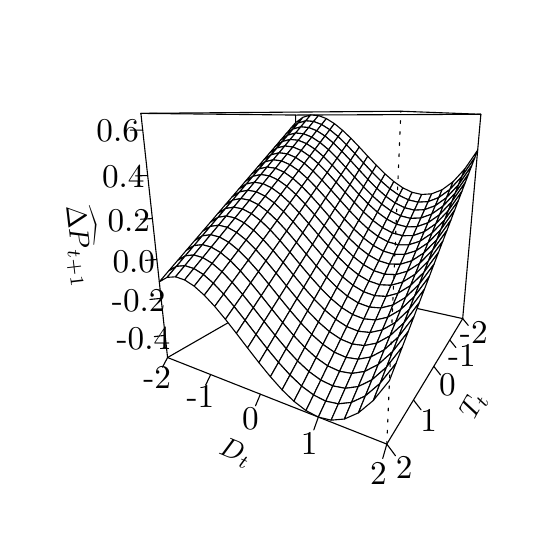
\begin{tikzpicture}[x=1pt,y=1pt]
\definecolor{fillColor}{RGB}{255,255,255}
\path[use as bounding box,fill=fillColor,fill opacity=0.00] (0,0) rectangle (180.67,180.67);
\begin{scope}
\path[clip] ( 36.00,  0.00) rectangle (168.67,180.67);
\definecolor{drawColor}{RGB}{0,0,0}

\path[draw=drawColor,line width= 0.4pt,line join=round,line cap=round] ( 97.94, 88.71) -- ( 96.79,149.09);

\path[draw=drawColor,line width= 0.4pt,line join=round,line cap=round] ( 96.79,149.09) -- ( 40.91,149.70);

\path[draw=drawColor,line width= 0.4pt,line join=round,line cap=round] ( 40.91,149.70) -- ( 50.55, 61.47);

\path[draw=drawColor,line width= 0.4pt,line join=round,line cap=round] ( 50.55, 61.47) -- ( 97.94, 88.71);

\path[draw=drawColor,line width= 0.4pt,line join=round,line cap=round] ( 97.94, 88.71) -- (157.19, 75.54);

\path[draw=drawColor,line width= 0.4pt,line join=round,line cap=round] (157.19, 75.54) -- (163.76,149.37);

\path[draw=drawColor,line width= 0.4pt,line join=round,line cap=round] (163.76,149.37) -- ( 96.79,149.09);

\path[draw=drawColor,line width= 0.4pt,line join=round,line cap=round] ( 50.55, 61.47) -- (129.77, 30.20);

\path[draw=drawColor,line width= 0.4pt,line join=round,line cap=round] (129.77, 30.20) -- (157.19, 75.54);

\path[draw=drawColor,line width= 0.4pt,line join=round,line cap=round] (163.76,149.37) -- (134.86,150.48);

\path[draw=drawColor,line width= 0.4pt,line join=round,line cap=round] (134.86,150.48) -- ( 40.91,149.70);
\end{scope}
\begin{scope}
\path[clip] (  0.00,  0.00) rectangle (180.67,180.67);
\definecolor{drawColor}{RGB}{0,0,0}

\node[text=drawColor,rotate= 60.83,anchor=base,inner sep=0pt, outer sep=0pt, scale=  1.00] at (153.16, 48.59) {};

\node[text=drawColor,rotate= 60.83,anchor=base,inner sep=0pt, outer sep=0pt, scale=  1.00] at (163.63, 42.74) { $T_{t}$};

\path[draw=drawColor,line width= 0.4pt,line join=round,line cap=round] (157.19, 75.54) -- (159.19, 73.10);

\node[text=drawColor,anchor=base,inner sep=0pt, outer sep=0pt, scale=  1.20] at (161.21, 66.51) {-2};

\path[draw=drawColor,line width= 0.4pt,line join=round,line cap=round] (152.52, 67.83) -- (154.73, 65.10);

\node[text=drawColor,anchor=base,inner sep=0pt, outer sep=0pt, scale=  1.20] at (156.95, 58.22) {-1};

\path[draw=drawColor,line width= 0.4pt,line join=round,line cap=round] (146.75, 58.28) -- (149.19, 55.18);

\node[text=drawColor,anchor=base,inner sep=0pt, outer sep=0pt, scale=  1.20] at (151.66, 47.93) {0};

\path[draw=drawColor,line width= 0.4pt,line join=round,line cap=round] (139.41, 46.14) -- (142.15, 42.57);

\node[text=drawColor,anchor=base,inner sep=0pt, outer sep=0pt, scale=  1.20] at (144.92, 34.84) {1};

\path[draw=drawColor,line width= 0.4pt,line join=round,line cap=round] (129.77, 30.20) -- (132.90, 25.99);

\node[text=drawColor,anchor=base,inner sep=0pt, outer sep=0pt, scale=  1.20] at (136.06, 17.60) {2};

\node[text=drawColor,rotate=-22.50,anchor=base,inner sep=0pt, outer sep=0pt, scale=  1.00] at ( 78.74, 35.52) {};

\node[text=drawColor,rotate=-22.50,anchor=base,inner sep=0pt, outer sep=0pt, scale=  1.00] at ( 74.15, 24.43) { $D_{t}$};

\path[draw=drawColor,line width= 0.4pt,line join=round,line cap=round] ( 50.55, 61.47) -- ( 48.70, 57.97);

\node[text=drawColor,anchor=base,inner sep=0pt, outer sep=0pt, scale=  1.20] at ( 46.82, 50.27) {-2};

\path[draw=drawColor,line width= 0.4pt,line join=round,line cap=round] ( 66.13, 55.32) -- ( 64.31, 51.50);

\node[text=drawColor,anchor=base,inner sep=0pt, outer sep=0pt, scale=  1.20] at ( 62.45, 43.48) {-1};

\path[draw=drawColor,line width= 0.4pt,line join=round,line cap=round] ( 84.09, 48.22) -- ( 82.33, 44.04);

\node[text=drawColor,anchor=base,inner sep=0pt, outer sep=0pt, scale=  1.20] at ( 80.53, 35.63) {0};

\path[draw=drawColor,line width= 0.4pt,line join=round,line cap=round] (105.04, 39.96) -- (103.38, 35.32);

\node[text=drawColor,anchor=base,inner sep=0pt, outer sep=0pt, scale=  1.20] at (101.69, 26.44) {1};

\path[draw=drawColor,line width= 0.4pt,line join=round,line cap=round] (129.77, 30.20) -- (128.29, 25.01);

\node[text=drawColor,anchor=base,inner sep=0pt, outer sep=0pt, scale=  1.20] at (126.77, 15.55) {2};

\node[text=drawColor,rotate=-83.36,anchor=base,inner sep=0pt, outer sep=0pt, scale=  1.00] at ( 39.50,104.20) {};

\node[text=drawColor,rotate=-83.36,anchor=base,inner sep=0pt, outer sep=0pt, scale=  1.00] at ( 27.58,102.81) {};

\node[text=drawColor,rotate=-83.36,anchor=base,inner sep=0pt, outer sep=0pt, scale=  1.00] at ( 15.66,101.42) { $\widehat{\Delta P}_{t+1}$};

\path[draw=drawColor,line width= 0.4pt,line join=round,line cap=round] ( 49.67, 69.50) -- ( 45.76, 69.03);

\node[text=drawColor,anchor=base,inner sep=0pt, outer sep=0pt, scale=  1.20] at ( 41.81, 64.42) {-0.4};

\path[draw=drawColor,line width= 0.4pt,line join=round,line cap=round] ( 48.21, 82.86) -- ( 44.20, 82.46);

\node[text=drawColor,anchor=base,inner sep=0pt, outer sep=0pt, scale=  1.20] at ( 40.13, 77.93) {-0.2};

\path[draw=drawColor,line width= 0.4pt,line join=round,line cap=round] ( 46.68, 96.90) -- ( 42.55, 96.58);

\node[text=drawColor,anchor=base,inner sep=0pt, outer sep=0pt, scale=  1.20] at ( 38.37, 92.13) {0.0};

\path[draw=drawColor,line width= 0.4pt,line join=round,line cap=round] ( 45.06,111.68) -- ( 40.82,111.45);

\node[text=drawColor,anchor=base,inner sep=0pt, outer sep=0pt, scale=  1.20] at ( 36.52,107.08) {0.2};

\path[draw=drawColor,line width= 0.4pt,line join=round,line cap=round] ( 43.36,127.24) -- ( 39.00,127.11);

\node[text=drawColor,anchor=base,inner sep=0pt, outer sep=0pt, scale=  1.20] at ( 34.57,122.84) {0.4};

\path[draw=drawColor,line width= 0.4pt,line join=round,line cap=round] ( 41.57,143.67) -- ( 37.07,143.64);

\node[text=drawColor,anchor=base,inner sep=0pt, outer sep=0pt, scale=  1.20] at ( 32.51,139.48) {0.6};
\end{scope}
\begin{scope}
\path[clip] ( 36.00,  0.00) rectangle (168.67,180.67);
\definecolor{drawColor}{RGB}{0,0,0}
\definecolor{fillColor}{RGB}{255,255,255}

\path[draw=drawColor,line width= 0.4pt,line join=round,line cap=round,fill=fillColor] ( 96.84,146.37) --
	( 95.04,144.27) --
	( 97.72,146.20) --
	( 99.50,148.30) --
	cycle;

\path[draw=drawColor,line width= 0.4pt,line join=round,line cap=round,fill=fillColor] ( 99.50,148.30) --
	( 97.72,146.20) --
	(100.48,147.00) --
	(102.24,149.11) --
	cycle;

\path[draw=drawColor,line width= 0.4pt,line join=round,line cap=round,fill=fillColor] ( 95.04,144.27) --
	( 93.19,142.11) --
	( 95.88,144.04) --
	( 97.72,146.20) --
	cycle;

\path[draw=drawColor,line width= 0.4pt,line join=round,line cap=round,fill=fillColor] (102.24,149.11) --
	(100.48,147.00) --
	(103.32,146.77) --
	(105.06,148.91) --
	cycle;

\path[draw=drawColor,line width= 0.4pt,line join=round,line cap=round,fill=fillColor] ( 97.72,146.20) --
	( 95.88,144.04) --
	( 98.67,144.82) --
	(100.48,147.00) --
	cycle;

\path[draw=drawColor,line width= 0.4pt,line join=round,line cap=round,fill=fillColor] (105.06,148.91) --
	(103.32,146.77) --
	(106.22,145.65) --
	(107.93,147.82) --
	cycle;

\path[draw=drawColor,line width= 0.4pt,line join=round,line cap=round,fill=fillColor] ( 93.19,142.11) --
	( 91.29,139.89) --
	( 93.99,141.82) --
	( 95.88,144.04) --
	cycle;

\path[draw=drawColor,line width= 0.4pt,line join=round,line cap=round,fill=fillColor] (100.48,147.00) --
	( 98.67,144.82) --
	(101.53,144.57) --
	(103.32,146.77) --
	cycle;

\path[draw=drawColor,line width= 0.4pt,line join=round,line cap=round,fill=fillColor] (107.93,147.82) --
	(106.22,145.65) --
	(109.17,143.78) --
	(110.85,145.99) --
	cycle;

\path[draw=drawColor,line width= 0.4pt,line join=round,line cap=round,fill=fillColor] ( 95.88,144.04) --
	( 93.99,141.82) --
	( 96.80,142.59) --
	( 98.67,144.82) --
	cycle;

\path[draw=drawColor,line width= 0.4pt,line join=round,line cap=round,fill=fillColor] (103.32,146.77) --
	(101.53,144.57) --
	(104.46,143.42) --
	(106.22,145.65) --
	cycle;

\path[draw=drawColor,line width= 0.4pt,line join=round,line cap=round,fill=fillColor] (110.85,145.99) --
	(109.17,143.78) --
	(112.17,141.30) --
	(113.81,143.56) --
	cycle;

\path[draw=drawColor,line width= 0.4pt,line join=round,line cap=round,fill=fillColor] ( 91.29,139.89) --
	( 89.33,137.60) --
	( 92.05,139.53) --
	( 93.99,141.82) --
	cycle;

\path[draw=drawColor,line width= 0.4pt,line join=round,line cap=round,fill=fillColor] ( 98.67,144.82) --
	( 96.80,142.59) --
	( 99.68,142.31) --
	(101.53,144.57) --
	cycle;

\path[draw=drawColor,line width= 0.4pt,line join=round,line cap=round,fill=fillColor] (106.22,145.65) --
	(104.46,143.42) --
	(107.44,141.50) --
	(109.17,143.78) --
	cycle;

\path[draw=drawColor,line width= 0.4pt,line join=round,line cap=round,fill=fillColor] (113.81,143.56) --
	(112.17,141.30) --
	(115.20,138.36) --
	(116.81,140.69) --
	cycle;

\path[draw=drawColor,line width= 0.4pt,line join=round,line cap=round,fill=fillColor] ( 93.99,141.82) --
	( 92.05,139.53) --
	( 94.87,140.28) --
	( 96.80,142.59) --
	cycle;

\path[draw=drawColor,line width= 0.4pt,line join=round,line cap=round,fill=fillColor] (101.53,144.57) --
	( 99.68,142.31) --
	(102.64,141.11) --
	(104.46,143.42) --
	cycle;

\path[draw=drawColor,line width= 0.4pt,line join=round,line cap=round,fill=fillColor] (109.17,143.78) --
	(107.44,141.50) --
	(110.47,138.96) --
	(112.17,141.30) --
	cycle;

\path[draw=drawColor,line width= 0.4pt,line join=round,line cap=round,fill=fillColor] ( 89.33,137.60) --
	( 87.31,135.25) --
	( 90.04,137.17) --
	( 92.05,139.53) --
	cycle;

\path[draw=drawColor,line width= 0.4pt,line join=round,line cap=round,fill=fillColor] (116.81,140.69) --
	(115.20,138.36) --
	(118.26,135.13) --
	(119.84,137.52) --
	cycle;

\path[draw=drawColor,line width= 0.4pt,line join=round,line cap=round,fill=fillColor] ( 96.80,142.59) --
	( 94.87,140.28) --
	( 97.78,139.97) --
	( 99.68,142.31) --
	cycle;

\path[draw=drawColor,line width= 0.4pt,line join=round,line cap=round,fill=fillColor] (104.46,143.42) --
	(102.64,141.11) --
	(105.65,139.14) --
	(107.44,141.50) --
	cycle;

\path[draw=drawColor,line width= 0.4pt,line join=round,line cap=round,fill=fillColor] (112.17,141.30) --
	(110.47,138.96) --
	(113.54,135.97) --
	(115.20,138.36) --
	cycle;

\path[draw=drawColor,line width= 0.4pt,line join=round,line cap=round,fill=fillColor] ( 92.05,139.53) --
	( 90.04,137.17) --
	( 92.88,137.90) --
	( 94.87,140.28) --
	cycle;

\path[draw=drawColor,line width= 0.4pt,line join=round,line cap=round,fill=fillColor] (119.84,137.52) --
	(118.26,135.13) --
	(121.36,131.76) --
	(122.90,134.21) --
	cycle;

\path[draw=drawColor,line width= 0.4pt,line join=round,line cap=round,fill=fillColor] ( 99.68,142.31) --
	( 97.78,139.97) --
	(100.77,138.74) --
	(102.64,141.11) --
	cycle;

\path[draw=drawColor,line width= 0.4pt,line join=round,line cap=round,fill=fillColor] (107.44,141.50) --
	(105.65,139.14) --
	(108.72,136.55) --
	(110.47,138.96) --
	cycle;

\path[draw=drawColor,line width= 0.4pt,line join=round,line cap=round,fill=fillColor] ( 87.31,135.25) --
	( 85.23,132.82) --
	( 87.98,134.73) --
	( 90.04,137.17) --
	cycle;

\path[draw=drawColor,line width= 0.4pt,line join=round,line cap=round,fill=fillColor] (115.20,138.36) --
	(113.54,135.97) --
	(116.64,132.67) --
	(118.26,135.13) --
	cycle;

\path[draw=drawColor,line width= 0.4pt,line join=round,line cap=round,fill=fillColor] ( 94.87,140.28) --
	( 92.88,137.90) --
	( 95.82,137.56) --
	( 97.78,139.97) --
	cycle;

\path[draw=drawColor,line width= 0.4pt,line join=round,line cap=round,fill=fillColor] (122.90,134.21) --
	(121.36,131.76) --
	(124.49,128.41) --
	(125.99,130.93) --
	cycle;

\path[draw=drawColor,line width= 0.4pt,line join=round,line cap=round,fill=fillColor] (102.64,141.11) --
	(100.77,138.74) --
	(103.81,136.72) --
	(105.65,139.14) --
	cycle;

\path[draw=drawColor,line width= 0.4pt,line join=round,line cap=round,fill=fillColor] (110.47,138.96) --
	(108.72,136.55) --
	(111.82,133.50) --
	(113.54,135.97) --
	cycle;

\path[draw=drawColor,line width= 0.4pt,line join=round,line cap=round,fill=fillColor] ( 90.04,137.17) --
	( 87.98,134.73) --
	( 90.83,135.44) --
	( 92.88,137.90) --
	cycle;

\path[draw=drawColor,line width= 0.4pt,line join=round,line cap=round,fill=fillColor] (118.26,135.13) --
	(116.64,132.67) --
	(119.77,129.24) --
	(121.36,131.76) --
	cycle;

\path[draw=drawColor,line width= 0.4pt,line join=round,line cap=round,fill=fillColor] ( 97.78,139.97) --
	( 95.82,137.56) --
	( 98.83,136.28) --
	(100.77,138.74) --
	cycle;

\path[draw=drawColor,line width= 0.4pt,line join=round,line cap=round,fill=fillColor] (125.99,130.93) --
	(124.49,128.41) --
	(127.67,125.24) --
	(129.13,127.82) --
	cycle;

\path[draw=drawColor,line width= 0.4pt,line join=round,line cap=round,fill=fillColor] (105.65,139.14) --
	(103.81,136.72) --
	(106.91,134.07) --
	(108.72,136.55) --
	cycle;

\path[draw=drawColor,line width= 0.4pt,line join=round,line cap=round,fill=fillColor] ( 85.23,132.82) --
	( 83.09,130.31) --
	( 85.84,132.22) --
	( 87.98,134.73) --
	cycle;

\path[draw=drawColor,line width= 0.4pt,line join=round,line cap=round,fill=fillColor] (113.54,135.97) --
	(111.82,133.50) --
	(114.96,130.13) --
	(116.64,132.67) --
	cycle;

\path[draw=drawColor,line width= 0.4pt,line join=round,line cap=round,fill=fillColor] ( 92.88,137.90) --
	( 90.83,135.44) --
	( 93.79,135.07) --
	( 95.82,137.56) --
	cycle;

\path[draw=drawColor,line width= 0.4pt,line join=round,line cap=round,fill=fillColor] (121.36,131.76) --
	(119.77,129.24) --
	(122.95,125.82) --
	(124.49,128.41) --
	cycle;

\path[draw=drawColor,line width= 0.4pt,line join=round,line cap=round,fill=fillColor] (100.77,138.74) --
	( 98.83,136.28) --
	(101.91,134.21) --
	(103.81,136.72) --
	cycle;

\path[draw=drawColor,line width= 0.4pt,line join=round,line cap=round,fill=fillColor] (129.13,127.82) --
	(127.67,125.24) --
	(130.90,122.41) --
	(132.32,125.05) --
	cycle;

\path[draw=drawColor,line width= 0.4pt,line join=round,line cap=round,fill=fillColor] (108.72,136.55) --
	(106.91,134.07) --
	(110.05,130.94) --
	(111.82,133.50) --
	cycle;

\path[draw=drawColor,line width= 0.4pt,line join=round,line cap=round,fill=fillColor] ( 87.98,134.73) --
	( 85.84,132.22) --
	( 88.72,132.91) --
	( 90.83,135.44) --
	cycle;

\path[draw=drawColor,line width= 0.4pt,line join=round,line cap=round,fill=fillColor] (116.64,132.67) --
	(114.96,130.13) --
	(118.14,126.63) --
	(119.77,129.24) --
	cycle;

\path[draw=drawColor,line width= 0.4pt,line join=round,line cap=round,fill=fillColor] ( 95.82,137.56) --
	( 93.79,135.07) --
	( 96.84,133.75) --
	( 98.83,136.28) --
	cycle;

\path[draw=drawColor,line width= 0.4pt,line join=round,line cap=round,fill=fillColor] (124.49,128.41) --
	(122.95,125.82) --
	(126.17,122.58) --
	(127.67,125.24) --
	cycle;

\path[draw=drawColor,line width= 0.4pt,line join=round,line cap=round,fill=fillColor] (103.81,136.72) --
	(101.91,134.21) --
	(105.05,131.50) --
	(106.91,134.07) --
	cycle;

\path[draw=drawColor,line width= 0.4pt,line join=round,line cap=round,fill=fillColor] (132.32,125.05) --
	(130.90,122.41) --
	(134.20,120.08) --
	(135.58,122.78) --
	cycle;

\path[draw=drawColor,line width= 0.4pt,line join=round,line cap=round,fill=fillColor] ( 83.09,130.31) --
	( 80.88,127.73) --
	( 83.64,129.63) --
	( 85.84,132.22) --
	cycle;

\path[draw=drawColor,line width= 0.4pt,line join=round,line cap=round,fill=fillColor] (111.82,133.50) --
	(110.05,130.94) --
	(113.23,127.51) --
	(114.96,130.13) --
	cycle;

\path[draw=drawColor,line width= 0.4pt,line join=round,line cap=round,fill=fillColor] ( 90.83,135.44) --
	( 88.72,132.91) --
	( 91.70,132.51) --
	( 93.79,135.07) --
	cycle;

\path[draw=drawColor,line width= 0.4pt,line join=round,line cap=round,fill=fillColor] (119.77,129.24) --
	(118.14,126.63) --
	(121.36,123.14) --
	(122.95,125.82) --
	cycle;

\path[draw=drawColor,line width= 0.4pt,line join=round,line cap=round,fill=fillColor] ( 98.83,136.28) --
	( 96.84,133.75) --
	( 99.95,131.63) --
	(101.91,134.21) --
	cycle;

\path[draw=drawColor,line width= 0.4pt,line join=round,line cap=round,fill=fillColor] (127.67,125.24) --
	(126.17,122.58) --
	(129.44,119.69) --
	(130.90,122.41) --
	cycle;

\path[draw=drawColor,line width= 0.4pt,line join=round,line cap=round,fill=fillColor] (106.91,134.07) --
	(105.05,131.50) --
	(108.23,128.31) --
	(110.05,130.94) --
	cycle;

\path[draw=drawColor,line width= 0.4pt,line join=round,line cap=round,fill=fillColor] (135.58,122.78) --
	(134.20,120.08) --
	(137.59,118.42) --
	(138.93,121.17) --
	cycle;

\path[draw=drawColor,line width= 0.4pt,line join=round,line cap=round,fill=fillColor] ( 85.84,132.22) --
	( 83.64,129.63) --
	( 86.54,130.30) --
	( 88.72,132.91) --
	cycle;

\path[draw=drawColor,line width= 0.4pt,line join=round,line cap=round,fill=fillColor] (114.96,130.13) --
	(113.23,127.51) --
	(116.45,123.94) --
	(118.14,126.63) --
	cycle;

\path[draw=drawColor,line width= 0.4pt,line join=round,line cap=round,fill=fillColor] ( 93.79,135.07) --
	( 91.70,132.51) --
	( 94.78,131.14) --
	( 96.84,133.75) --
	cycle;

\path[draw=drawColor,line width= 0.4pt,line join=round,line cap=round,fill=fillColor] (122.95,125.82) --
	(121.36,123.14) --
	(124.62,119.84) --
	(126.17,122.58) --
	cycle;

\path[draw=drawColor,line width= 0.4pt,line join=round,line cap=round,fill=fillColor] (101.91,134.21) --
	( 99.95,131.63) --
	(103.12,128.85) --
	(105.05,131.50) --
	cycle;

\path[draw=drawColor,line width= 0.4pt,line join=round,line cap=round,fill=fillColor] (130.90,122.41) --
	(129.44,119.69) --
	(132.78,117.30) --
	(134.20,120.08) --
	cycle;

\path[draw=drawColor,line width= 0.4pt,line join=round,line cap=round,fill=fillColor] ( 80.88,127.73) --
	( 78.59,125.06) --
	( 81.37,126.95) --
	( 83.64,129.63) --
	cycle;

\path[draw=drawColor,line width= 0.4pt,line join=round,line cap=round,fill=fillColor] (110.05,130.94) --
	(108.23,128.31) --
	(111.45,124.81) --
	(113.23,127.51) --
	cycle;

\path[draw=drawColor,line width= 0.4pt,line join=round,line cap=round,fill=fillColor] (138.93,121.17) --
	(137.59,118.42) --
	(141.09,117.60) --
	(142.38,120.39) --
	cycle;

\path[draw=drawColor,line width= 0.4pt,line join=round,line cap=round,fill=fillColor] ( 88.72,132.91) --
	( 86.54,130.30) --
	( 89.54,129.85) --
	( 91.70,132.51) --
	cycle;

\path[draw=drawColor,line width= 0.4pt,line join=round,line cap=round,fill=fillColor] (118.14,126.63) --
	(116.45,123.94) --
	(119.71,120.38) --
	(121.36,123.14) --
	cycle;

\path[draw=drawColor,line width= 0.4pt,line join=round,line cap=round,fill=fillColor] ( 96.84,133.75) --
	( 94.78,131.14) --
	( 97.92,128.96) --
	( 99.95,131.63) --
	cycle;

\path[draw=drawColor,line width= 0.4pt,line join=round,line cap=round,fill=fillColor] (126.17,122.58) --
	(124.62,119.84) --
	(127.93,116.88) --
	(129.44,119.69) --
	cycle;

\path[draw=drawColor,line width= 0.4pt,line join=round,line cap=round,fill=fillColor] (105.05,131.50) --
	(103.12,128.85) --
	(106.34,125.59) --
	(108.23,128.31) --
	cycle;

\path[draw=drawColor,line width= 0.4pt,line join=round,line cap=round,fill=fillColor] (134.20,120.08) --
	(132.78,117.30) --
	(136.21,115.58) --
	(137.59,118.42) --
	cycle;

\path[draw=drawColor,line width= 0.4pt,line join=round,line cap=round,fill=fillColor] ( 83.64,129.63) --
	( 81.37,126.95) --
	( 84.28,127.59) --
	( 86.54,130.30) --
	cycle;

\path[draw=drawColor,line width= 0.4pt,line join=round,line cap=round,fill=fillColor] (113.23,127.51) --
	(111.45,124.81) --
	(114.71,121.16) --
	(116.45,123.94) --
	cycle;

\path[draw=drawColor,line width= 0.4pt,line join=round,line cap=round,fill=fillColor] (142.38,120.39) --
	(141.09,117.60) --
	(144.72,117.81) --
	(145.98,120.63) --
	cycle;

\path[draw=drawColor,line width= 0.4pt,line join=round,line cap=round,fill=fillColor] ( 91.70,132.51) --
	( 89.54,129.85) --
	( 92.65,128.44) --
	( 94.78,131.14) --
	cycle;

\path[draw=drawColor,line width= 0.4pt,line join=round,line cap=round,fill=fillColor] (121.36,123.14) --
	(119.71,120.38) --
	(123.01,117.00) --
	(124.62,119.84) --
	cycle;

\path[draw=drawColor,line width= 0.4pt,line join=round,line cap=round,fill=fillColor] ( 99.95,131.63) --
	( 97.92,128.96) --
	(101.13,126.11) --
	(103.12,128.85) --
	cycle;

\path[draw=drawColor,line width= 0.4pt,line join=round,line cap=round,fill=fillColor] (129.44,119.69) --
	(127.93,116.88) --
	(131.31,114.42) --
	(132.78,117.30) --
	cycle;

\path[draw=drawColor,line width= 0.4pt,line join=round,line cap=round,fill=fillColor] ( 78.59,125.06) --
	( 76.23,122.30) --
	( 79.02,124.18) --
	( 81.37,126.95) --
	cycle;

\path[draw=drawColor,line width= 0.4pt,line join=round,line cap=round,fill=fillColor] (108.23,128.31) --
	(106.34,125.59) --
	(109.60,122.01) --
	(111.45,124.81) --
	cycle;

\path[draw=drawColor,line width= 0.4pt,line join=round,line cap=round,fill=fillColor] (137.59,118.42) --
	(136.21,115.58) --
	(139.75,114.72) --
	(141.09,117.60) --
	cycle;

\path[draw=drawColor,line width= 0.4pt,line join=round,line cap=round,fill=fillColor] ( 86.54,130.30) --
	( 84.28,127.59) --
	( 87.31,127.11) --
	( 89.54,129.85) --
	cycle;

\path[draw=drawColor,line width= 0.4pt,line join=round,line cap=round,fill=fillColor] (116.45,123.94) --
	(114.71,121.16) --
	(118.01,117.52) --
	(119.71,120.38) --
	cycle;

\path[draw=drawColor,line width= 0.4pt,line join=round,line cap=round,fill=fillColor] (145.98,120.63) --
	(144.72,117.81) --
	(148.54,119.26) --
	(149.75,122.10) --
	cycle;

\path[draw=drawColor,line width= 0.4pt,line join=round,line cap=round,fill=fillColor] ( 94.78,131.14) --
	( 92.65,128.44) --
	( 95.83,126.19) --
	( 97.92,128.96) --
	cycle;

\path[draw=drawColor,line width= 0.4pt,line join=round,line cap=round,fill=fillColor] (124.62,119.84) --
	(123.01,117.00) --
	(126.37,113.97) --
	(127.93,116.88) --
	cycle;

\path[draw=drawColor,line width= 0.4pt,line join=round,line cap=round,fill=fillColor] (103.12,128.85) --
	(101.13,126.11) --
	(104.39,122.78) --
	(106.34,125.59) --
	cycle;

\path[draw=drawColor,line width= 0.4pt,line join=round,line cap=round,fill=fillColor] (132.78,117.30) --
	(131.31,114.42) --
	(134.78,112.65) --
	(136.21,115.58) --
	cycle;

\path[draw=drawColor,line width= 0.4pt,line join=round,line cap=round,fill=fillColor] ( 81.37,126.95) --
	( 79.02,124.18) --
	( 81.95,124.80) --
	( 84.28,127.59) --
	cycle;

\path[draw=drawColor,line width= 0.4pt,line join=round,line cap=round,fill=fillColor] (111.45,124.81) --
	(109.60,122.01) --
	(112.91,118.28) --
	(114.71,121.16) --
	cycle;

\path[draw=drawColor,line width= 0.4pt,line join=round,line cap=round,fill=fillColor] (141.09,117.60) --
	(139.75,114.72) --
	(143.43,114.90) --
	(144.72,117.81) --
	cycle;

\path[draw=drawColor,line width= 0.4pt,line join=round,line cap=round,fill=fillColor] ( 89.54,129.85) --
	( 87.31,127.11) --
	( 90.44,125.64) --
	( 92.65,128.44) --
	cycle;

\path[draw=drawColor,line width= 0.4pt,line join=round,line cap=round,fill=fillColor] (119.71,120.38) --
	(118.01,117.52) --
	(121.36,114.07) --
	(123.01,117.00) --
	cycle;

\path[draw=drawColor,line width= 0.4pt,line join=round,line cap=round,fill=fillColor] (149.75,122.10) --
	(148.54,119.26) --
	(152.57,122.19) --
	(153.74,125.03) --
	cycle;

\path[draw=drawColor,line width= 0.4pt,line join=round,line cap=round,fill=fillColor] ( 97.92,128.96) --
	( 95.83,126.19) --
	( 99.07,123.28) --
	(101.13,126.11) --
	cycle;

\path[draw=drawColor,line width= 0.4pt,line join=round,line cap=round,fill=fillColor] (127.93,116.88) --
	(126.37,113.97) --
	(129.80,111.45) --
	(131.31,114.42) --
	cycle;

\path[draw=drawColor,line width= 0.4pt,line join=round,line cap=round,fill=fillColor] ( 76.23,122.30) --
	( 73.79,119.45) --
	( 76.59,121.32) --
	( 79.02,124.18) --
	cycle;

\path[draw=drawColor,line width= 0.4pt,line join=round,line cap=round,fill=fillColor] (106.34,125.59) --
	(104.39,122.78) --
	(107.70,119.12) --
	(109.60,122.01) --
	cycle;

\path[draw=drawColor,line width= 0.4pt,line join=round,line cap=round,fill=fillColor] (136.21,115.58) --
	(134.78,112.65) --
	(138.37,111.74) --
	(139.75,114.72) --
	cycle;

\path[draw=drawColor,line width= 0.4pt,line join=round,line cap=round,fill=fillColor] ( 84.28,127.59) --
	( 81.95,124.80) --
	( 85.00,124.28) --
	( 87.31,127.11) --
	cycle;

\path[draw=drawColor,line width= 0.4pt,line join=round,line cap=round,fill=fillColor] (114.71,121.16) --
	(112.91,118.28) --
	(116.25,114.57) --
	(118.01,117.52) --
	cycle;

\path[draw=drawColor,line width= 0.4pt,line join=round,line cap=round,fill=fillColor] (144.72,117.81) --
	(143.43,114.90) --
	(147.29,116.33) --
	(148.54,119.26) --
	cycle;

\path[draw=drawColor,line width= 0.4pt,line join=round,line cap=round,fill=fillColor] ( 92.65,128.44) --
	( 90.44,125.64) --
	( 93.66,123.34) --
	( 95.83,126.19) --
	cycle;

\path[draw=drawColor,line width= 0.4pt,line join=round,line cap=round,fill=fillColor] (123.01,117.00) --
	(121.36,114.07) --
	(124.76,110.97) --
	(126.37,113.97) --
	cycle;

\path[draw=drawColor,line width= 0.4pt,line join=round,line cap=round,fill=fillColor] (153.74,125.03) --
	(152.57,122.19) --
	(156.89,126.88) --
	(158.00,129.69) --
	cycle;

\path[draw=drawColor,line width= 0.4pt,line join=round,line cap=round,fill=fillColor] (101.13,126.11) --
	( 99.07,123.28) --
	(102.38,119.88) --
	(104.39,122.78) --
	cycle;

\path[draw=drawColor,line width= 0.4pt,line join=round,line cap=round,fill=fillColor] (131.31,114.42) --
	(129.80,111.45) --
	(133.31,109.63) --
	(134.78,112.65) --
	cycle;

\path[draw=drawColor,line width= 0.4pt,line join=round,line cap=round,fill=fillColor] ( 79.02,124.18) --
	( 76.59,121.32) --
	( 79.53,121.91) --
	( 81.95,124.80) --
	cycle;

\path[draw=drawColor,line width= 0.4pt,line join=round,line cap=round,fill=fillColor] (109.60,122.01) --
	(107.70,119.12) --
	(111.04,115.31) --
	(112.91,118.28) --
	cycle;

\path[draw=drawColor,line width= 0.4pt,line join=round,line cap=round,fill=fillColor] (139.75,114.72) --
	(138.37,111.74) --
	(142.09,111.89) --
	(143.43,114.90) --
	cycle;

\path[draw=drawColor,line width= 0.4pt,line join=round,line cap=round,fill=fillColor] ( 87.31,127.11) --
	( 85.00,124.28) --
	( 88.17,122.76) --
	( 90.44,125.64) --
	cycle;

\path[draw=drawColor,line width= 0.4pt,line join=round,line cap=round,fill=fillColor] (118.01,117.52) --
	(116.25,114.57) --
	(119.64,111.04) --
	(121.36,114.07) --
	cycle;

\path[draw=drawColor,line width= 0.4pt,line join=round,line cap=round,fill=fillColor] (148.54,119.26) --
	(147.29,116.33) --
	(151.37,119.26) --
	(152.57,122.19) --
	cycle;

\path[draw=drawColor,line width= 0.4pt,line join=round,line cap=round,fill=fillColor] ( 95.83,126.19) --
	( 93.66,123.34) --
	( 96.95,120.36) --
	( 99.07,123.28) --
	cycle;

\path[draw=drawColor,line width= 0.4pt,line join=round,line cap=round,fill=fillColor] (126.37,113.97) --
	(124.76,110.97) --
	(128.23,108.38) --
	(129.80,111.45) --
	cycle;

\path[draw=drawColor,line width= 0.4pt,line join=round,line cap=round,fill=fillColor] (158.00,129.69) --
	(156.89,126.88) --
	(161.55,133.65) --
	(162.61,136.42) --
	cycle;

\path[draw=drawColor,line width= 0.4pt,line join=round,line cap=round,fill=fillColor] ( 73.79,119.45) --
	( 71.27,116.51) --
	( 74.07,118.36) --
	( 76.59,121.32) --
	cycle;

\path[draw=drawColor,line width= 0.4pt,line join=round,line cap=round,fill=fillColor] (104.39,122.78) --
	(102.38,119.88) --
	(105.73,116.14) --
	(107.70,119.12) --
	cycle;

\path[draw=drawColor,line width= 0.4pt,line join=round,line cap=round,fill=fillColor] (134.78,112.65) --
	(133.31,109.63) --
	(136.94,108.67) --
	(138.37,111.74) --
	cycle;

\path[draw=drawColor,line width= 0.4pt,line join=round,line cap=round,fill=fillColor] ( 81.95,124.80) --
	( 79.53,121.91) --
	( 82.61,121.35) --
	( 85.00,124.28) --
	cycle;

\path[draw=drawColor,line width= 0.4pt,line join=round,line cap=round,fill=fillColor] (112.91,118.28) --
	(111.04,115.31) --
	(114.43,111.52) --
	(116.25,114.57) --
	cycle;

\path[draw=drawColor,line width= 0.4pt,line join=round,line cap=round,fill=fillColor] (143.43,114.90) --
	(142.09,111.89) --
	(146.00,113.30) --
	(147.29,116.33) --
	cycle;

\path[draw=drawColor,line width= 0.4pt,line join=round,line cap=round,fill=fillColor] ( 90.44,125.64) --
	( 88.17,122.76) --
	( 91.42,120.38) --
	( 93.66,123.34) --
	cycle;

\path[draw=drawColor,line width= 0.4pt,line join=round,line cap=round,fill=fillColor] (121.36,114.07) --
	(119.64,111.04) --
	(123.09,107.86) --
	(124.76,110.97) --
	cycle;

\path[draw=drawColor,line width= 0.4pt,line join=round,line cap=round,fill=fillColor] (152.57,122.19) --
	(151.37,119.26) --
	(155.73,123.96) --
	(156.89,126.88) --
	cycle;

\path[draw=drawColor,line width= 0.4pt,line join=round,line cap=round,fill=fillColor] ( 99.07,123.28) --
	( 96.95,120.36) --
	(100.29,116.87) --
	(102.38,119.88) --
	cycle;

\path[draw=drawColor,line width= 0.4pt,line join=round,line cap=round,fill=fillColor] (129.80,111.45) --
	(128.23,108.38) --
	(131.79,106.49) --
	(133.31,109.63) --
	cycle;

\path[draw=drawColor,line width= 0.4pt,line join=round,line cap=round,fill=fillColor] ( 76.59,121.32) --
	( 74.07,118.36) --
	( 77.04,118.92) --
	( 79.53,121.91) --
	cycle;

\path[draw=drawColor,line width= 0.4pt,line join=round,line cap=round,fill=fillColor] (107.70,119.12) --
	(105.73,116.14) --
	(109.12,112.24) --
	(111.04,115.31) --
	cycle;

\path[draw=drawColor,line width= 0.4pt,line join=round,line cap=round,fill=fillColor] (138.37,111.74) --
	(136.94,108.67) --
	(140.71,108.77) --
	(142.09,111.89) --
	cycle;

\path[draw=drawColor,line width= 0.4pt,line join=round,line cap=round,fill=fillColor] ( 85.00,124.28) --
	( 82.61,121.35) --
	( 85.81,119.77) --
	( 88.17,122.76) --
	cycle;

\path[draw=drawColor,line width= 0.4pt,line join=round,line cap=round,fill=fillColor] (116.25,114.57) --
	(114.43,111.52) --
	(117.87,107.90) --
	(119.64,111.04) --
	cycle;

\path[draw=drawColor,line width= 0.4pt,line join=round,line cap=round,fill=fillColor] (147.29,116.33) --
	(146.00,113.30) --
	(150.13,116.22) --
	(151.37,119.26) --
	cycle;

\path[draw=drawColor,line width= 0.4pt,line join=round,line cap=round,fill=fillColor] ( 93.66,123.34) --
	( 91.42,120.38) --
	( 94.74,117.33) --
	( 96.95,120.36) --
	cycle;

\path[draw=drawColor,line width= 0.4pt,line join=round,line cap=round,fill=fillColor] (124.76,110.97) --
	(123.09,107.86) --
	(126.61,105.21) --
	(128.23,108.38) --
	cycle;

\path[draw=drawColor,line width= 0.4pt,line join=round,line cap=round,fill=fillColor] (156.89,126.88) --
	(155.73,123.96) --
	(160.45,130.78) --
	(161.55,133.65) --
	cycle;

\path[draw=drawColor,line width= 0.4pt,line join=round,line cap=round,fill=fillColor] ( 71.27,116.51) --
	( 68.67,113.47) --
	( 71.47,115.30) --
	( 74.07,118.36) --
	cycle;

\path[draw=drawColor,line width= 0.4pt,line join=round,line cap=round,fill=fillColor] (102.38,119.88) --
	(100.29,116.87) --
	(103.68,113.04) --
	(105.73,116.14) --
	cycle;

\path[draw=drawColor,line width= 0.4pt,line join=round,line cap=round,fill=fillColor] (133.31,109.63) --
	(131.79,106.49) --
	(135.46,105.48) --
	(136.94,108.67) --
	cycle;

\path[draw=drawColor,line width= 0.4pt,line join=round,line cap=round,fill=fillColor] ( 79.53,121.91) --
	( 77.04,118.92) --
	( 80.14,118.31) --
	( 82.61,121.35) --
	cycle;

\path[draw=drawColor,line width= 0.4pt,line join=round,line cap=round,fill=fillColor] (111.04,115.31) --
	(109.12,112.24) --
	(112.55,108.36) --
	(114.43,111.52) --
	cycle;

\path[draw=drawColor,line width= 0.4pt,line join=round,line cap=round,fill=fillColor] (142.09,111.89) --
	(140.71,108.77) --
	(144.66,110.16) --
	(146.00,113.30) --
	cycle;

\path[draw=drawColor,line width= 0.4pt,line join=round,line cap=round,fill=fillColor] ( 88.17,122.76) --
	( 85.81,119.77) --
	( 89.10,117.32) --
	( 91.42,120.38) --
	cycle;

\path[draw=drawColor,line width= 0.4pt,line join=round,line cap=round,fill=fillColor] (119.64,111.04) --
	(117.87,107.90) --
	(121.36,104.65) --
	(123.09,107.86) --
	cycle;

\path[draw=drawColor,line width= 0.4pt,line join=round,line cap=round,fill=fillColor] (151.37,119.26) --
	(150.13,116.22) --
	(154.54,120.94) --
	(155.73,123.96) --
	cycle;

\path[draw=drawColor,line width= 0.4pt,line join=round,line cap=round,fill=fillColor] ( 96.95,120.36) --
	( 94.74,117.33) --
	( 98.13,113.75) --
	(100.29,116.87) --
	cycle;

\path[draw=drawColor,line width= 0.4pt,line join=round,line cap=round,fill=fillColor] (128.23,108.38) --
	(126.61,105.21) --
	(130.21,103.25) --
	(131.79,106.49) --
	cycle;

\path[draw=drawColor,line width= 0.4pt,line join=round,line cap=round,fill=fillColor] ( 74.07,118.36) --
	( 71.47,115.30) --
	( 74.45,115.82) --
	( 77.04,118.92) --
	cycle;

\path[draw=drawColor,line width= 0.4pt,line join=round,line cap=round,fill=fillColor] (105.73,116.14) --
	(103.68,113.04) --
	(107.12,109.06) --
	(109.12,112.24) --
	cycle;

\path[draw=drawColor,line width= 0.4pt,line join=round,line cap=round,fill=fillColor] (136.94,108.67) --
	(135.46,105.48) --
	(139.28,105.54) --
	(140.71,108.77) --
	cycle;

\path[draw=drawColor,line width= 0.4pt,line join=round,line cap=round,fill=fillColor] ( 82.61,121.35) --
	( 80.14,118.31) --
	( 83.37,116.67) --
	( 85.81,119.77) --
	cycle;

\path[draw=drawColor,line width= 0.4pt,line join=round,line cap=round,fill=fillColor] (114.43,111.52) --
	(112.55,108.36) --
	(116.04,104.66) --
	(117.87,107.90) --
	cycle;

\path[draw=drawColor,line width= 0.4pt,line join=round,line cap=round,fill=fillColor] (146.00,113.30) --
	(144.66,110.16) --
	(148.84,113.07) --
	(150.13,116.22) --
	cycle;

\path[draw=drawColor,line width= 0.4pt,line join=round,line cap=round,fill=fillColor] ( 91.42,120.38) --
	( 89.10,117.32) --
	( 92.46,114.19) --
	( 94.74,117.33) --
	cycle;

\path[draw=drawColor,line width= 0.4pt,line join=round,line cap=round,fill=fillColor] (123.09,107.86) --
	(121.36,104.65) --
	(124.93,101.92) --
	(126.61,105.21) --
	cycle;

\path[draw=drawColor,line width= 0.4pt,line join=round,line cap=round,fill=fillColor] (155.73,123.96) --
	(154.54,120.94) --
	(159.31,127.81) --
	(160.45,130.78) --
	cycle;

\path[draw=drawColor,line width= 0.4pt,line join=round,line cap=round,fill=fillColor] ( 68.67,113.47) --
	( 65.97,110.31) --
	( 68.78,112.13) --
	( 71.47,115.30) --
	cycle;

\path[draw=drawColor,line width= 0.4pt,line join=round,line cap=round,fill=fillColor] (100.29,116.87) --
	( 98.13,113.75) --
	(101.57,109.84) --
	(103.68,113.04) --
	cycle;

\path[draw=drawColor,line width= 0.4pt,line join=round,line cap=round,fill=fillColor] (131.79,106.49) --
	(130.21,103.25) --
	(133.93,102.19) --
	(135.46,105.48) --
	cycle;

\path[draw=drawColor,line width= 0.4pt,line join=round,line cap=round,fill=fillColor] ( 77.04,118.92) --
	( 74.45,115.82) --
	( 77.58,115.16) --
	( 80.14,118.31) --
	cycle;

\path[draw=drawColor,line width= 0.4pt,line join=round,line cap=round,fill=fillColor] (109.12,112.24) --
	(107.12,109.06) --
	(110.61,105.09) --
	(112.55,108.36) --
	cycle;

\path[draw=drawColor,line width= 0.4pt,line join=round,line cap=round,fill=fillColor] (140.71,108.77) --
	(139.28,105.54) --
	(143.27,106.90) --
	(144.66,110.16) --
	cycle;

\path[draw=drawColor,line width= 0.4pt,line join=round,line cap=round,fill=fillColor] ( 85.81,119.77) --
	( 83.37,116.67) --
	( 86.69,114.16) --
	( 89.10,117.32) --
	cycle;

\path[draw=drawColor,line width= 0.4pt,line join=round,line cap=round,fill=fillColor] (117.87,107.90) --
	(116.04,104.66) --
	(119.58,101.32) --
	(121.36,104.65) --
	cycle;

\path[draw=drawColor,line width= 0.4pt,line join=round,line cap=round,fill=fillColor] (150.13,116.22) --
	(148.84,113.07) --
	(153.30,117.81) --
	(154.54,120.94) --
	cycle;

\path[draw=drawColor,line width= 0.4pt,line join=round,line cap=round,fill=fillColor] ( 94.74,117.33) --
	( 92.46,114.19) --
	( 95.89,110.53) --
	( 98.13,113.75) --
	cycle;

\path[draw=drawColor,line width= 0.4pt,line join=round,line cap=round,fill=fillColor] (126.61,105.21) --
	(124.93,101.92) --
	(128.58, 99.90) --
	(130.21,103.25) --
	cycle;

\path[draw=drawColor,line width= 0.4pt,line join=round,line cap=round,fill=fillColor] ( 71.47,115.30) --
	( 68.78,112.13) --
	( 71.77,112.62) --
	( 74.45,115.82) --
	cycle;

\path[draw=drawColor,line width= 0.4pt,line join=round,line cap=round,fill=fillColor] (103.68,113.04) --
	(101.57,109.84) --
	(105.06,105.76) --
	(107.12,109.06) --
	cycle;

\path[draw=drawColor,line width= 0.4pt,line join=round,line cap=round,fill=fillColor] (135.46,105.48) --
	(133.93,102.19) --
	(137.79,102.21) --
	(139.28,105.54) --
	cycle;

\path[draw=drawColor,line width= 0.4pt,line join=round,line cap=round,fill=fillColor] ( 80.14,118.31) --
	( 77.58,115.16) --
	( 80.84,113.46) --
	( 83.37,116.67) --
	cycle;

\path[draw=drawColor,line width= 0.4pt,line join=round,line cap=round,fill=fillColor] (112.55,108.36) --
	(110.61,105.09) --
	(114.14,101.30) --
	(116.04,104.66) --
	cycle;

\path[draw=drawColor,line width= 0.4pt,line join=round,line cap=round,fill=fillColor] (144.66,110.16) --
	(143.27,106.90) --
	(147.50,109.81) --
	(148.84,113.07) --
	cycle;

\path[draw=drawColor,line width= 0.4pt,line join=round,line cap=round,fill=fillColor] ( 89.10,117.32) --
	( 86.69,114.16) --
	( 90.10,110.94) --
	( 92.46,114.19) --
	cycle;

\path[draw=drawColor,line width= 0.4pt,line join=round,line cap=round,fill=fillColor] (121.36,104.65) --
	(119.58,101.32) --
	(123.19, 98.52) --
	(124.93,101.92) --
	cycle;

\path[draw=drawColor,line width= 0.4pt,line join=round,line cap=round,fill=fillColor] (154.54,120.94) --
	(153.30,117.81) --
	(158.13,124.73) --
	(159.31,127.81) --
	cycle;

\path[draw=drawColor,line width= 0.4pt,line join=round,line cap=round,fill=fillColor] ( 65.97,110.31) --
	( 63.17,107.05) --
	( 65.99,108.84) --
	( 68.78,112.13) --
	cycle;

\path[draw=drawColor,line width= 0.4pt,line join=round,line cap=round,fill=fillColor] ( 98.13,113.75) --
	( 95.89,110.53) --
	( 99.38,106.52) --
	(101.57,109.84) --
	cycle;

\path[draw=drawColor,line width= 0.4pt,line join=round,line cap=round,fill=fillColor] (130.21,103.25) --
	(128.58, 99.90) --
	(132.34, 98.77) --
	(133.93,102.19) --
	cycle;

\path[draw=drawColor,line width= 0.4pt,line join=round,line cap=round,fill=fillColor] ( 74.45,115.82) --
	( 71.77,112.62) --
	( 74.92,111.90) --
	( 77.58,115.16) --
	cycle;

\path[draw=drawColor,line width= 0.4pt,line join=round,line cap=round,fill=fillColor] (107.12,109.06) --
	(105.06,105.76) --
	(108.59,101.70) --
	(110.61,105.09) --
	cycle;

\path[draw=drawColor,line width= 0.4pt,line join=round,line cap=round,fill=fillColor] (139.28,105.54) --
	(137.79,102.21) --
	(141.84,103.53) --
	(143.27,106.90) --
	cycle;

\path[draw=drawColor,line width= 0.4pt,line join=round,line cap=round,fill=fillColor] ( 83.37,116.67) --
	( 80.84,113.46) --
	( 84.20,110.87) --
	( 86.69,114.16) --
	cycle;

\path[draw=drawColor,line width= 0.4pt,line join=round,line cap=round,fill=fillColor] (116.04,104.66) --
	(114.14,101.30) --
	(117.73, 97.88) --
	(119.58,101.32) --
	cycle;

\path[draw=drawColor,line width= 0.4pt,line join=round,line cap=round,fill=fillColor] (148.84,113.07) --
	(147.50,109.81) --
	(152.02,114.57) --
	(153.30,117.81) --
	cycle;

\path[draw=drawColor,line width= 0.4pt,line join=round,line cap=round,fill=fillColor] ( 92.46,114.19) --
	( 90.10,110.94) --
	( 93.58,107.19) --
	( 95.89,110.53) --
	cycle;

\path[draw=drawColor,line width= 0.4pt,line join=round,line cap=round,fill=fillColor] (124.93,101.92) --
	(123.19, 98.52) --
	(126.89, 96.42) --
	(128.58, 99.90) --
	cycle;

\path[draw=drawColor,line width= 0.4pt,line join=round,line cap=round,fill=fillColor] ( 68.78,112.13) --
	( 65.99,108.84) --
	( 69.00,109.29) --
	( 71.77,112.62) --
	cycle;

\path[draw=drawColor,line width= 0.4pt,line join=round,line cap=round,fill=fillColor] (101.57,109.84) --
	( 99.38,106.52) --
	(102.92,102.35) --
	(105.06,105.76) --
	cycle;

\path[draw=drawColor,line width= 0.4pt,line join=round,line cap=round,fill=fillColor] (133.93,102.19) --
	(132.34, 98.77) --
	(136.25, 98.74) --
	(137.79,102.21) --
	cycle;

\path[draw=drawColor,line width= 0.4pt,line join=round,line cap=round,fill=fillColor] ( 77.58,115.16) --
	( 74.92,111.90) --
	( 78.21,110.13) --
	( 80.84,113.46) --
	cycle;

\path[draw=drawColor,line width= 0.4pt,line join=round,line cap=round,fill=fillColor] (110.61,105.09) --
	(108.59,101.70) --
	(112.17, 97.82) --
	(114.14,101.30) --
	cycle;

\path[draw=drawColor,line width= 0.4pt,line join=round,line cap=round,fill=fillColor] (143.27,106.90) --
	(141.84,103.53) --
	(146.12,106.43) --
	(147.50,109.81) --
	cycle;

\path[draw=drawColor,line width= 0.4pt,line join=round,line cap=round,fill=fillColor] ( 86.69,114.16) --
	( 84.20,110.87) --
	( 87.65,107.56) --
	( 90.10,110.94) --
	cycle;

\path[draw=drawColor,line width= 0.4pt,line join=round,line cap=round,fill=fillColor] (119.58,101.32) --
	(117.73, 97.88) --
	(121.39, 94.99) --
	(123.19, 98.52) --
	cycle;

\path[draw=drawColor,line width= 0.4pt,line join=round,line cap=round,fill=fillColor] (153.30,117.81) --
	(152.02,114.57) --
	(156.91,121.53) --
	(158.13,124.73) --
	cycle;

\path[draw=drawColor,line width= 0.4pt,line join=round,line cap=round,fill=fillColor] ( 63.17,107.05) --
	( 60.28,103.67) --
	( 63.09,105.43) --
	( 65.99,108.84) --
	cycle;

\path[draw=drawColor,line width= 0.4pt,line join=round,line cap=round,fill=fillColor] ( 95.89,110.53) --
	( 93.58,107.19) --
	( 97.11,103.08) --
	( 99.38,106.52) --
	cycle;

\path[draw=drawColor,line width= 0.4pt,line join=round,line cap=round,fill=fillColor] (128.58, 99.90) --
	(126.89, 96.42) --
	(130.70, 95.24) --
	(132.34, 98.77) --
	cycle;

\path[draw=drawColor,line width= 0.4pt,line join=round,line cap=round,fill=fillColor] ( 71.77,112.62) --
	( 69.00,109.29) --
	( 72.17,108.52) --
	( 74.92,111.90) --
	cycle;

\path[draw=drawColor,line width= 0.4pt,line join=round,line cap=round,fill=fillColor] (105.06,105.76) --
	(102.92,102.35) --
	(106.50, 98.19) --
	(108.59,101.70) --
	cycle;

\path[draw=drawColor,line width= 0.4pt,line join=round,line cap=round,fill=fillColor] (137.79,102.21) --
	(136.25, 98.74) --
	(140.35,100.04) --
	(141.84,103.53) --
	cycle;

\path[draw=drawColor,line width= 0.4pt,line join=round,line cap=round,fill=fillColor] ( 80.84,113.46) --
	( 78.21,110.13) --
	( 81.61,107.46) --
	( 84.20,110.87) --
	cycle;

\path[draw=drawColor,line width= 0.4pt,line join=round,line cap=round,fill=fillColor] (114.14,101.30) --
	(112.17, 97.82) --
	(115.81, 94.31) --
	(117.73, 97.88) --
	cycle;

\path[draw=drawColor,line width= 0.4pt,line join=round,line cap=round,fill=fillColor] (147.50,109.81) --
	(146.12,106.43) --
	(150.69,111.20) --
	(152.02,114.57) --
	cycle;

\path[draw=drawColor,line width= 0.4pt,line join=round,line cap=round,fill=fillColor] ( 90.10,110.94) --
	( 87.65,107.56) --
	( 91.17,103.72) --
	( 93.58,107.19) --
	cycle;

\path[draw=drawColor,line width= 0.4pt,line join=round,line cap=round,fill=fillColor] (123.19, 98.52) --
	(121.39, 94.99) --
	(125.14, 92.82) --
	(126.89, 96.42) --
	cycle;

\path[draw=drawColor,line width= 0.4pt,line join=round,line cap=round,fill=fillColor] ( 65.99,108.84) --
	( 63.09,105.43) --
	( 66.11,105.84) --
	( 69.00,109.29) --
	cycle;

\path[draw=drawColor,line width= 0.4pt,line join=round,line cap=round,fill=fillColor] ( 99.38,106.52) --
	( 97.11,103.08) --
	(100.70, 98.81) --
	(102.92,102.35) --
	cycle;

\path[draw=drawColor,line width= 0.4pt,line join=round,line cap=round,fill=fillColor] (132.34, 98.77) --
	(130.70, 95.24) --
	(134.66, 95.16) --
	(136.25, 98.74) --
	cycle;

\path[draw=drawColor,line width= 0.4pt,line join=round,line cap=round,fill=fillColor] ( 74.92,111.90) --
	( 72.17,108.52) --
	( 75.49,106.68) --
	( 78.21,110.13) --
	cycle;

\path[draw=drawColor,line width= 0.4pt,line join=round,line cap=round,fill=fillColor] (108.59,101.70) --
	(106.50, 98.19) --
	(110.13, 94.21) --
	(112.17, 97.82) --
	cycle;

\path[draw=drawColor,line width= 0.4pt,line join=round,line cap=round,fill=fillColor] (141.84,103.53) --
	(140.35,100.04) --
	(144.68,102.92) --
	(146.12,106.43) --
	cycle;

\path[draw=drawColor,line width= 0.4pt,line join=round,line cap=round,fill=fillColor] ( 84.20,110.87) --
	( 81.61,107.46) --
	( 85.10,104.06) --
	( 87.65,107.56) --
	cycle;

\path[draw=drawColor,line width= 0.4pt,line join=round,line cap=round,fill=fillColor] (117.73, 97.88) --
	(115.81, 94.31) --
	(119.52, 91.33) --
	(121.39, 94.99) --
	cycle;

\path[draw=drawColor,line width= 0.4pt,line join=round,line cap=round,fill=fillColor] (152.02,114.57) --
	(150.69,111.20) --
	(155.64,118.21) --
	(156.91,121.53) --
	cycle;

\path[draw=drawColor,line width= 0.4pt,line join=round,line cap=round,fill=fillColor] ( 60.28,103.67) --
	( 57.28,100.16) --
	( 60.09,101.90) --
	( 63.09,105.43) --
	cycle;

\path[draw=drawColor,line width= 0.4pt,line join=round,line cap=round,fill=fillColor] ( 93.58,107.19) --
	( 91.17,103.72) --
	( 94.75, 99.51) --
	( 97.11,103.08) --
	cycle;

\path[draw=drawColor,line width= 0.4pt,line join=round,line cap=round,fill=fillColor] (126.89, 96.42) --
	(125.14, 92.82) --
	(129.00, 91.57) --
	(130.70, 95.24) --
	cycle;

\path[draw=drawColor,line width= 0.4pt,line join=round,line cap=round,fill=fillColor] ( 69.00,109.29) --
	( 66.11,105.84) --
	( 69.31,105.01) --
	( 72.17,108.52) --
	cycle;

\path[draw=drawColor,line width= 0.4pt,line join=round,line cap=round,fill=fillColor] (102.92,102.35) --
	(100.70, 98.81) --
	(104.33, 94.54) --
	(106.50, 98.19) --
	cycle;

\path[draw=drawColor,line width= 0.4pt,line join=round,line cap=round,fill=fillColor] (136.25, 98.74) --
	(134.66, 95.16) --
	(138.81, 96.42) --
	(140.35,100.04) --
	cycle;

\path[draw=drawColor,line width= 0.4pt,line join=round,line cap=round,fill=fillColor] ( 78.21,110.13) --
	( 75.49,106.68) --
	( 78.93,103.92) --
	( 81.61,107.46) --
	cycle;

\path[draw=drawColor,line width= 0.4pt,line join=round,line cap=round,fill=fillColor] (112.17, 97.82) --
	(110.13, 94.21) --
	(113.82, 90.60) --
	(115.81, 94.31) --
	cycle;

\path[draw=drawColor,line width= 0.4pt,line join=round,line cap=round,fill=fillColor] (146.12,106.43) --
	(144.68,102.92) --
	(149.31,107.70) --
	(150.69,111.20) --
	cycle;

\path[draw=drawColor,line width= 0.4pt,line join=round,line cap=round,fill=fillColor] ( 87.65,107.56) --
	( 85.10,104.06) --
	( 88.67,100.12) --
	( 91.17,103.72) --
	cycle;

\path[draw=drawColor,line width= 0.4pt,line join=round,line cap=round,fill=fillColor] (121.39, 94.99) --
	(119.52, 91.33) --
	(123.32, 89.09) --
	(125.14, 92.82) --
	cycle;

\path[draw=drawColor,line width= 0.4pt,line join=round,line cap=round,fill=fillColor] ( 63.09,105.43) --
	( 60.09,101.90) --
	( 63.12,102.26) --
	( 66.11,105.84) --
	cycle;

\path[draw=drawColor,line width= 0.4pt,line join=round,line cap=round,fill=fillColor] ( 97.11,103.08) --
	( 94.75, 99.51) --
	( 98.39, 95.13) --
	(100.70, 98.81) --
	cycle;

\path[draw=drawColor,line width= 0.4pt,line join=round,line cap=round,fill=fillColor] (130.70, 95.24) --
	(129.00, 91.57) --
	(133.01, 91.43) --
	(134.66, 95.16) --
	cycle;

\path[draw=drawColor,line width= 0.4pt,line join=round,line cap=round,fill=fillColor] ( 72.17,108.52) --
	( 69.31,105.01) --
	( 72.66,103.09) --
	( 75.49,106.68) --
	cycle;

\path[draw=drawColor,line width= 0.4pt,line join=round,line cap=round,fill=fillColor] (106.50, 98.19) --
	(104.33, 94.54) --
	(108.02, 90.47) --
	(110.13, 94.21) --
	cycle;

\path[draw=drawColor,line width= 0.4pt,line join=round,line cap=round,fill=fillColor] (140.35,100.04) --
	(138.81, 96.42) --
	(143.19, 99.28) --
	(144.68,102.92) --
	cycle;

\path[draw=drawColor,line width= 0.4pt,line join=round,line cap=round,fill=fillColor] ( 81.61,107.46) --
	( 78.93,103.92) --
	( 82.46,100.43) --
	( 85.10,104.06) --
	cycle;

\path[draw=drawColor,line width= 0.4pt,line join=round,line cap=round,fill=fillColor] (115.81, 94.31) --
	(113.82, 90.60) --
	(117.58, 87.54) --
	(119.52, 91.33) --
	cycle;

\path[draw=drawColor,line width= 0.4pt,line join=round,line cap=round,fill=fillColor] (150.69,111.20) --
	(149.31,107.70) --
	(154.31,114.75) --
	(155.64,118.21) --
	cycle;

\path[draw=drawColor,line width= 0.4pt,line join=round,line cap=round,fill=fillColor] ( 57.28,100.16) --
	( 54.16, 96.52) --
	( 56.97, 98.22) --
	( 60.09,101.90) --
	cycle;

\path[draw=drawColor,line width= 0.4pt,line join=round,line cap=round,fill=fillColor] ( 91.17,103.72) --
	( 88.67,100.12) --
	( 92.31, 95.81) --
	( 94.75, 99.51) --
	cycle;

\path[draw=drawColor,line width= 0.4pt,line join=round,line cap=round,fill=fillColor] (125.14, 92.82) --
	(123.32, 89.09) --
	(127.23, 87.76) --
	(129.00, 91.57) --
	cycle;

\path[draw=drawColor,line width= 0.4pt,line join=round,line cap=round,fill=fillColor] ( 66.11,105.84) --
	( 63.12,102.26) --
	( 66.34,101.36) --
	( 69.31,105.01) --
	cycle;

\path[draw=drawColor,line width= 0.4pt,line join=round,line cap=round,fill=fillColor] (100.70, 98.81) --
	( 98.39, 95.13) --
	(102.08, 90.76) --
	(104.33, 94.54) --
	cycle;

\path[draw=drawColor,line width= 0.4pt,line join=round,line cap=round,fill=fillColor] (134.66, 95.16) --
	(133.01, 91.43) --
	(137.20, 92.65) --
	(138.81, 96.42) --
	cycle;

\path[draw=drawColor,line width= 0.4pt,line join=round,line cap=round,fill=fillColor] ( 75.49,106.68) --
	( 72.66,103.09) --
	( 76.14,100.25) --
	( 78.93,103.92) --
	cycle;

\path[draw=drawColor,line width= 0.4pt,line join=round,line cap=round,fill=fillColor] (110.13, 94.21) --
	(108.02, 90.47) --
	(111.76, 86.76) --
	(113.82, 90.60) --
	cycle;

\path[draw=drawColor,line width= 0.4pt,line join=round,line cap=round,fill=fillColor] (144.68,102.92) --
	(143.19, 99.28) --
	(147.87,104.07) --
	(149.31,107.70) --
	cycle;

\path[draw=drawColor,line width= 0.4pt,line join=round,line cap=round,fill=fillColor] ( 85.10,104.06) --
	( 82.46,100.43) --
	( 86.08, 96.38) --
	( 88.67,100.12) --
	cycle;

\path[draw=drawColor,line width= 0.4pt,line join=round,line cap=round,fill=fillColor] (119.52, 91.33) --
	(117.58, 87.54) --
	(121.43, 85.21) --
	(123.32, 89.09) --
	cycle;

\path[draw=drawColor,line width= 0.4pt,line join=round,line cap=round,fill=fillColor] ( 60.09,101.90) --
	( 56.97, 98.22) --
	( 60.01, 98.53) --
	( 63.12,102.26) --
	cycle;

\path[draw=drawColor,line width= 0.4pt,line join=round,line cap=round,fill=fillColor] ( 94.75, 99.51) --
	( 92.31, 95.81) --
	( 96.00, 91.32) --
	( 98.39, 95.13) --
	cycle;

\path[draw=drawColor,line width= 0.4pt,line join=round,line cap=round,fill=fillColor] (129.00, 91.57) --
	(127.23, 87.76) --
	(131.29, 87.57) --
	(133.01, 91.43) --
	cycle;

\path[draw=drawColor,line width= 0.4pt,line join=round,line cap=round,fill=fillColor] ( 69.31,105.01) --
	( 66.34,101.36) --
	( 69.72, 99.37) --
	( 72.66,103.09) --
	cycle;

\path[draw=drawColor,line width= 0.4pt,line join=round,line cap=round,fill=fillColor] (104.33, 94.54) --
	(102.08, 90.76) --
	(105.82, 86.58) --
	(108.02, 90.47) --
	cycle;

\path[draw=drawColor,line width= 0.4pt,line join=round,line cap=round,fill=fillColor] (138.81, 96.42) --
	(137.20, 92.65) --
	(141.64, 95.50) --
	(143.19, 99.28) --
	cycle;

\path[draw=drawColor,line width= 0.4pt,line join=round,line cap=round,fill=fillColor] ( 78.93,103.92) --
	( 76.14,100.25) --
	( 79.72, 96.65) --
	( 82.46,100.43) --
	cycle;

\path[draw=drawColor,line width= 0.4pt,line join=round,line cap=round,fill=fillColor] (113.82, 90.60) --
	(111.76, 86.76) --
	(115.57, 83.60) --
	(117.58, 87.54) --
	cycle;

\path[draw=drawColor,line width= 0.4pt,line join=round,line cap=round,fill=fillColor] (149.31,107.70) --
	(147.87,104.07) --
	(152.94,111.16) --
	(154.31,114.75) --
	cycle;

\path[draw=drawColor,line width= 0.4pt,line join=round,line cap=round,fill=fillColor] ( 54.16, 96.52) --
	( 50.92, 92.74) --
	( 53.73, 94.41) --
	( 56.97, 98.22) --
	cycle;

\path[draw=drawColor,line width= 0.4pt,line join=round,line cap=round,fill=fillColor] ( 88.67,100.12) --
	( 86.08, 96.38) --
	( 89.77, 91.96) --
	( 92.31, 95.81) --
	cycle;

\path[draw=drawColor,line width= 0.4pt,line join=round,line cap=round,fill=fillColor] (123.32, 89.09) --
	(121.43, 85.21) --
	(125.40, 83.81) --
	(127.23, 87.76) --
	cycle;

\path[draw=drawColor,line width= 0.4pt,line join=round,line cap=round,fill=fillColor] ( 63.12,102.26) --
	( 60.01, 98.53) --
	( 63.26, 97.57) --
	( 66.34,101.36) --
	cycle;

\path[draw=drawColor,line width= 0.4pt,line join=round,line cap=round,fill=fillColor] ( 98.39, 95.13) --
	( 96.00, 91.32) --
	( 99.74, 86.83) --
	(102.08, 90.76) --
	cycle;

\path[draw=drawColor,line width= 0.4pt,line join=round,line cap=round,fill=fillColor] (133.01, 91.43) --
	(131.29, 87.57) --
	(135.54, 88.74) --
	(137.20, 92.65) --
	cycle;

\path[draw=drawColor,line width= 0.4pt,line join=round,line cap=round,fill=fillColor] ( 72.66,103.09) --
	( 69.72, 99.37) --
	( 73.24, 96.43) --
	( 76.14,100.25) --
	cycle;

\path[draw=drawColor,line width= 0.4pt,line join=round,line cap=round,fill=fillColor] (108.02, 90.47) --
	(105.82, 86.58) --
	(109.61, 82.76) --
	(111.76, 86.76) --
	cycle;

\path[draw=drawColor,line width= 0.4pt,line join=round,line cap=round,fill=fillColor] (143.19, 99.28) --
	(141.64, 95.50) --
	(146.38,100.29) --
	(147.87,104.07) --
	cycle;

\path[draw=drawColor,line width= 0.4pt,line join=round,line cap=round,fill=fillColor] ( 82.46,100.43) --
	( 79.72, 96.65) --
	( 83.39, 92.49) --
	( 86.08, 96.38) --
	cycle;

\path[draw=drawColor,line width= 0.4pt,line join=round,line cap=round,fill=fillColor] (117.58, 87.54) --
	(115.57, 83.60) --
	(119.47, 81.18) --
	(121.43, 85.21) --
	cycle;

\path[draw=drawColor,line width= 0.4pt,line join=round,line cap=round,fill=fillColor] ( 56.97, 98.22) --
	( 53.73, 94.41) --
	( 56.78, 94.66) --
	( 60.01, 98.53) --
	cycle;

\path[draw=drawColor,line width= 0.4pt,line join=round,line cap=round,fill=fillColor] ( 92.31, 95.81) --
	( 89.77, 91.96) --
	( 93.51, 87.35) --
	( 96.00, 91.32) --
	cycle;

\path[draw=drawColor,line width= 0.4pt,line join=round,line cap=round,fill=fillColor] (127.23, 87.76) --
	(125.40, 83.81) --
	(129.51, 83.55) --
	(131.29, 87.57) --
	cycle;

\path[draw=drawColor,line width= 0.4pt,line join=round,line cap=round,fill=fillColor] ( 66.34,101.36) --
	( 63.26, 97.57) --
	( 66.67, 95.49) --
	( 69.72, 99.37) --
	cycle;

\path[draw=drawColor,line width= 0.4pt,line join=round,line cap=round,fill=fillColor] (102.08, 90.76) --
	( 99.74, 86.83) --
	(103.53, 82.54) --
	(105.82, 86.58) --
	cycle;

\path[draw=drawColor,line width= 0.4pt,line join=round,line cap=round,fill=fillColor] (137.20, 92.65) --
	(135.54, 88.74) --
	(140.03, 91.56) --
	(141.64, 95.50) --
	cycle;

\path[draw=drawColor,line width= 0.4pt,line join=round,line cap=round,fill=fillColor] ( 76.14,100.25) --
	( 73.24, 96.43) --
	( 76.86, 92.73) --
	( 79.72, 96.65) --
	cycle;

\path[draw=drawColor,line width= 0.4pt,line join=round,line cap=round,fill=fillColor] (111.76, 86.76) --
	(109.61, 82.76) --
	(113.48, 79.50) --
	(115.57, 83.60) --
	cycle;

\path[draw=drawColor,line width= 0.4pt,line join=round,line cap=round,fill=fillColor] (147.87,104.07) --
	(146.38,100.29) --
	(151.51,107.42) --
	(152.94,111.16) --
	cycle;

\path[draw=drawColor,line width= 0.4pt,line join=round,line cap=round,fill=fillColor] ( 50.92, 92.74) --
	( 47.56, 88.81) --
	( 50.36, 90.44) --
	( 53.73, 94.41) --
	cycle;

\path[draw=drawColor,line width= 0.4pt,line join=round,line cap=round,fill=fillColor] ( 86.08, 96.38) --
	( 83.39, 92.49) --
	( 87.13, 87.96) --
	( 89.77, 91.96) --
	cycle;

\path[draw=drawColor,line width= 0.4pt,line join=round,line cap=round,fill=fillColor] (121.43, 85.21) --
	(119.47, 81.18) --
	(123.49, 79.70) --
	(125.40, 83.81) --
	cycle;

\path[draw=drawColor,line width= 0.4pt,line join=round,line cap=round,fill=fillColor] ( 60.01, 98.53) --
	( 56.78, 94.66) --
	( 60.04, 93.63) --
	( 63.26, 97.57) --
	cycle;

\path[draw=drawColor,line width= 0.4pt,line join=round,line cap=round,fill=fillColor] ( 96.00, 91.32) --
	( 93.51, 87.35) --
	( 97.31, 82.75) --
	( 99.74, 86.83) --
	cycle;

\path[draw=drawColor,line width= 0.4pt,line join=round,line cap=round,fill=fillColor] (131.29, 87.57) --
	(129.51, 83.55) --
	(133.81, 84.68) --
	(135.54, 88.74) --
	cycle;

\path[draw=drawColor,line width= 0.4pt,line join=round,line cap=round,fill=fillColor] ( 69.72, 99.37) --
	( 66.67, 95.49) --
	( 70.22, 92.45) --
	( 73.24, 96.43) --
	cycle;

\path[draw=drawColor,line width= 0.4pt,line join=round,line cap=round,fill=fillColor] (105.82, 86.58) --
	(103.53, 82.54) --
	(107.38, 78.61) --
	(109.61, 82.76) --
	cycle;

\path[draw=drawColor,line width= 0.4pt,line join=round,line cap=round,fill=fillColor] (141.64, 95.50) --
	(140.03, 91.56) --
	(144.82, 96.36) --
	(146.38,100.29) --
	cycle;

\path[draw=drawColor,line width= 0.4pt,line join=round,line cap=round,fill=fillColor] ( 79.72, 96.65) --
	( 76.86, 92.73) --
	( 80.58, 88.45) --
	( 83.39, 92.49) --
	cycle;

\path[draw=drawColor,line width= 0.4pt,line join=round,line cap=round,fill=fillColor] (115.57, 83.60) --
	(113.48, 79.50) --
	(117.44, 76.99) --
	(119.47, 81.18) --
	cycle;

\path[draw=drawColor,line width= 0.4pt,line join=round,line cap=round,fill=fillColor] ( 53.73, 94.41) --
	( 50.36, 90.44) --
	( 53.42, 90.64) --
	( 56.78, 94.66) --
	cycle;

\path[draw=drawColor,line width= 0.4pt,line join=round,line cap=round,fill=fillColor] ( 89.77, 91.96) --
	( 87.13, 87.96) --
	( 90.93, 83.23) --
	( 93.51, 87.35) --
	cycle;

\path[draw=drawColor,line width= 0.4pt,line join=round,line cap=round,fill=fillColor] (125.40, 83.81) --
	(123.49, 79.70) --
	(127.65, 79.37) --
	(129.51, 83.55) --
	cycle;

\path[draw=drawColor,line width= 0.4pt,line join=round,line cap=round,fill=fillColor] ( 63.26, 97.57) --
	( 60.04, 93.63) --
	( 63.49, 91.46) --
	( 66.67, 95.49) --
	cycle;

\path[draw=drawColor,line width= 0.4pt,line join=round,line cap=round,fill=fillColor] ( 99.74, 86.83) --
	( 97.31, 82.75) --
	(101.16, 78.33) --
	(103.53, 82.54) --
	cycle;

\path[draw=drawColor,line width= 0.4pt,line join=round,line cap=round,fill=fillColor] (135.54, 88.74) --
	(133.81, 84.68) --
	(138.35, 87.47) --
	(140.03, 91.56) --
	cycle;

\path[draw=drawColor,line width= 0.4pt,line join=round,line cap=round,fill=fillColor] ( 73.24, 96.43) --
	( 70.22, 92.45) --
	( 73.89, 88.64) --
	( 76.86, 92.73) --
	cycle;

\path[draw=drawColor,line width= 0.4pt,line join=round,line cap=round,fill=fillColor] (109.61, 82.76) --
	(107.38, 78.61) --
	(111.31, 75.25) --
	(113.48, 79.50) --
	cycle;

\path[draw=drawColor,line width= 0.4pt,line join=round,line cap=round,fill=fillColor] (146.38,100.29) --
	(144.82, 96.36) --
	(150.01,103.52) --
	(151.51,107.42) --
	cycle;

\path[draw=drawColor,line width= 0.4pt,line join=round,line cap=round,fill=fillColor] ( 83.39, 92.49) --
	( 80.58, 88.45) --
	( 84.38, 83.79) --
	( 87.13, 87.96) --
	cycle;

\path[draw=drawColor,line width= 0.4pt,line join=round,line cap=round,fill=fillColor] (119.47, 81.18) --
	(117.44, 76.99) --
	(121.50, 75.43) --
	(123.49, 79.70) --
	cycle;

\path[draw=drawColor,line width= 0.4pt,line join=round,line cap=round,fill=fillColor] ( 56.78, 94.66) --
	( 53.42, 90.64) --
	( 56.70, 89.53) --
	( 60.04, 93.63) --
	cycle;

\path[draw=drawColor,line width= 0.4pt,line join=round,line cap=round,fill=fillColor] ( 93.51, 87.35) --
	( 90.93, 83.23) --
	( 94.78, 78.50) --
	( 97.31, 82.75) --
	cycle;

\path[draw=drawColor,line width= 0.4pt,line join=round,line cap=round,fill=fillColor] (129.51, 83.55) --
	(127.65, 79.37) --
	(132.00, 80.45) --
	(133.81, 84.68) --
	cycle;

\path[draw=drawColor,line width= 0.4pt,line join=round,line cap=round,fill=fillColor] ( 66.67, 95.49) --
	( 63.49, 91.46) --
	( 67.08, 88.32) --
	( 70.22, 92.45) --
	cycle;

\path[draw=drawColor,line width= 0.4pt,line join=round,line cap=round,fill=fillColor] (103.53, 82.54) --
	(101.16, 78.33) --
	(105.07, 74.29) --
	(107.38, 78.61) --
	cycle;

\path[draw=drawColor,line width= 0.4pt,line join=round,line cap=round,fill=fillColor] (140.03, 91.56) --
	(138.35, 87.47) --
	(143.20, 92.26) --
	(144.82, 96.36) --
	cycle;

\path[draw=drawColor,line width= 0.4pt,line join=round,line cap=round,fill=fillColor] ( 76.86, 92.73) --
	( 73.89, 88.64) --
	( 77.66, 84.24) --
	( 80.58, 88.45) --
	cycle;

\path[draw=drawColor,line width= 0.4pt,line join=round,line cap=round,fill=fillColor] (113.48, 79.50) --
	(111.31, 75.25) --
	(115.32, 72.64) --
	(117.44, 76.99) --
	cycle;

\path[draw=drawColor,line width= 0.4pt,line join=round,line cap=round,fill=fillColor] ( 87.13, 87.96) --
	( 84.38, 83.79) --
	( 88.23, 78.93) --
	( 90.93, 83.23) --
	cycle;

\path[draw=drawColor,line width= 0.4pt,line join=round,line cap=round,fill=fillColor] (123.49, 79.70) --
	(121.50, 75.43) --
	(125.72, 75.03) --
	(127.65, 79.37) --
	cycle;

\path[draw=drawColor,line width= 0.4pt,line join=round,line cap=round,fill=fillColor] ( 60.04, 93.63) --
	( 56.70, 89.53) --
	( 60.17, 87.26) --
	( 63.49, 91.46) --
	cycle;

\path[draw=drawColor,line width= 0.4pt,line join=round,line cap=round,fill=fillColor] ( 97.31, 82.75) --
	( 94.78, 78.50) --
	( 98.69, 73.96) --
	(101.16, 78.33) --
	cycle;

\path[draw=drawColor,line width= 0.4pt,line join=round,line cap=round,fill=fillColor] (133.81, 84.68) --
	(132.00, 80.45) --
	(136.60, 83.21) --
	(138.35, 87.47) --
	cycle;

\path[draw=drawColor,line width= 0.4pt,line join=round,line cap=round,fill=fillColor] ( 70.22, 92.45) --
	( 67.08, 88.32) --
	( 70.80, 84.38) --
	( 73.89, 88.64) --
	cycle;

\path[draw=drawColor,line width= 0.4pt,line join=round,line cap=round,fill=fillColor] (107.38, 78.61) --
	(105.07, 74.29) --
	(109.04, 70.82) --
	(111.31, 75.25) --
	cycle;

\path[draw=drawColor,line width= 0.4pt,line join=round,line cap=round,fill=fillColor] (144.82, 96.36) --
	(143.20, 92.26) --
	(148.46, 99.46) --
	(150.01,103.52) --
	cycle;

\path[draw=drawColor,line width= 0.4pt,line join=round,line cap=round,fill=fillColor] ( 80.58, 88.45) --
	( 77.66, 84.24) --
	( 81.51, 79.45) --
	( 84.38, 83.79) --
	cycle;

\path[draw=drawColor,line width= 0.4pt,line join=round,line cap=round,fill=fillColor] (117.44, 76.99) --
	(115.32, 72.64) --
	(119.44, 70.98) --
	(121.50, 75.43) --
	cycle;

\path[draw=drawColor,line width= 0.4pt,line join=round,line cap=round,fill=fillColor] ( 90.93, 83.23) --
	( 88.23, 78.93) --
	( 92.15, 74.08) --
	( 94.78, 78.50) --
	cycle;

\path[draw=drawColor,line width= 0.4pt,line join=round,line cap=round,fill=fillColor] (127.65, 79.37) --
	(125.72, 75.03) --
	(130.13, 76.04) --
	(132.00, 80.45) --
	cycle;

\path[draw=drawColor,line width= 0.4pt,line join=round,line cap=round,fill=fillColor] ( 63.49, 91.46) --
	( 60.17, 87.26) --
	( 63.81, 84.00) --
	( 67.08, 88.32) --
	cycle;

\path[draw=drawColor,line width= 0.4pt,line join=round,line cap=round,fill=fillColor] (101.16, 78.33) --
	( 98.69, 73.96) --
	(102.65, 69.80) --
	(105.07, 74.29) --
	cycle;

\path[draw=drawColor,line width= 0.4pt,line join=round,line cap=round,fill=fillColor] (138.35, 87.47) --
	(136.60, 83.21) --
	(141.51, 87.99) --
	(143.20, 92.26) --
	cycle;

\path[draw=drawColor,line width= 0.4pt,line join=round,line cap=round,fill=fillColor] ( 73.89, 88.64) --
	( 70.80, 84.38) --
	( 74.62, 79.86) --
	( 77.66, 84.24) --
	cycle;

\path[draw=drawColor,line width= 0.4pt,line join=round,line cap=round,fill=fillColor] (111.31, 75.25) --
	(109.04, 70.82) --
	(113.11, 68.10) --
	(115.32, 72.64) --
	cycle;

\path[draw=drawColor,line width= 0.4pt,line join=round,line cap=round,fill=fillColor] ( 84.38, 83.79) --
	( 81.51, 79.45) --
	( 85.43, 74.46) --
	( 88.23, 78.93) --
	cycle;

\path[draw=drawColor,line width= 0.4pt,line join=round,line cap=round,fill=fillColor] (121.50, 75.43) --
	(119.44, 70.98) --
	(123.71, 70.50) --
	(125.72, 75.03) --
	cycle;

\path[draw=drawColor,line width= 0.4pt,line join=round,line cap=round,fill=fillColor] ( 94.78, 78.50) --
	( 92.15, 74.08) --
	( 96.11, 69.41) --
	( 98.69, 73.96) --
	cycle;

\path[draw=drawColor,line width= 0.4pt,line join=round,line cap=round,fill=fillColor] (132.00, 80.45) --
	(130.13, 76.04) --
	(134.78, 78.76) --
	(136.60, 83.21) --
	cycle;

\path[draw=drawColor,line width= 0.4pt,line join=round,line cap=round,fill=fillColor] ( 67.08, 88.32) --
	( 63.81, 84.00) --
	( 67.58, 79.95) --
	( 70.80, 84.38) --
	cycle;

\path[draw=drawColor,line width= 0.4pt,line join=round,line cap=round,fill=fillColor] (105.07, 74.29) --
	(102.65, 69.80) --
	(106.69, 66.21) --
	(109.04, 70.82) --
	cycle;

\path[draw=drawColor,line width= 0.4pt,line join=round,line cap=round,fill=fillColor] (143.20, 92.26) --
	(141.51, 87.99) --
	(146.83, 95.22) --
	(148.46, 99.46) --
	cycle;

\path[draw=drawColor,line width= 0.4pt,line join=round,line cap=round,fill=fillColor] ( 77.66, 84.24) --
	( 74.62, 79.86) --
	( 78.53, 74.93) --
	( 81.51, 79.45) --
	cycle;

\path[draw=drawColor,line width= 0.4pt,line join=round,line cap=round,fill=fillColor] (115.32, 72.64) --
	(113.11, 68.10) --
	(117.29, 66.35) --
	(119.44, 70.98) --
	cycle;

\path[draw=drawColor,line width= 0.4pt,line join=round,line cap=round,fill=fillColor] ( 88.23, 78.93) --
	( 85.43, 74.46) --
	( 89.40, 69.47) --
	( 92.15, 74.08) --
	cycle;

\path[draw=drawColor,line width= 0.4pt,line join=round,line cap=round,fill=fillColor] (125.72, 75.03) --
	(123.71, 70.50) --
	(128.17, 71.45) --
	(130.13, 76.04) --
	cycle;

\path[draw=drawColor,line width= 0.4pt,line join=round,line cap=round,fill=fillColor] ( 98.69, 73.96) --
	( 96.11, 69.41) --
	(100.14, 65.12) --
	(102.65, 69.80) --
	cycle;

\path[draw=drawColor,line width= 0.4pt,line join=round,line cap=round,fill=fillColor] (136.60, 83.21) --
	(134.78, 78.76) --
	(139.75, 83.53) --
	(141.51, 87.99) --
	cycle;

\path[draw=drawColor,line width= 0.4pt,line join=round,line cap=round,fill=fillColor] ( 70.80, 84.38) --
	( 67.58, 79.95) --
	( 71.45, 75.29) --
	( 74.62, 79.86) --
	cycle;

\path[draw=drawColor,line width= 0.4pt,line join=round,line cap=round,fill=fillColor] (109.04, 70.82) --
	(106.69, 66.21) --
	(110.81, 63.38) --
	(113.11, 68.10) --
	cycle;

\path[draw=drawColor,line width= 0.4pt,line join=round,line cap=round,fill=fillColor] ( 81.51, 79.45) --
	( 78.53, 74.93) --
	( 82.50, 69.80) --
	( 85.43, 74.46) --
	cycle;

\path[draw=drawColor,line width= 0.4pt,line join=round,line cap=round,fill=fillColor] (119.44, 70.98) --
	(117.29, 66.35) --
	(121.62, 65.78) --
	(123.71, 70.50) --
	cycle;

\path[draw=drawColor,line width= 0.4pt,line join=round,line cap=round,fill=fillColor] ( 92.15, 74.08) --
	( 89.40, 69.47) --
	( 93.43, 64.66) --
	( 96.11, 69.41) --
	cycle;

\path[draw=drawColor,line width= 0.4pt,line join=round,line cap=round,fill=fillColor] (130.13, 76.04) --
	(128.17, 71.45) --
	(132.88, 74.13) --
	(134.78, 78.76) --
	cycle;

\path[draw=drawColor,line width= 0.4pt,line join=round,line cap=round,fill=fillColor] (102.65, 69.80) --
	(100.14, 65.12) --
	(104.23, 61.40) --
	(106.69, 66.21) --
	cycle;

\path[draw=drawColor,line width= 0.4pt,line join=round,line cap=round,fill=fillColor] (141.51, 87.99) --
	(139.75, 83.53) --
	(145.14, 90.78) --
	(146.83, 95.22) --
	cycle;

\path[draw=drawColor,line width= 0.4pt,line join=round,line cap=round,fill=fillColor] ( 74.62, 79.86) --
	( 71.45, 75.29) --
	( 75.42, 70.21) --
	( 78.53, 74.93) --
	cycle;

\path[draw=drawColor,line width= 0.4pt,line join=round,line cap=round,fill=fillColor] (113.11, 68.10) --
	(110.81, 63.38) --
	(115.05, 61.52) --
	(117.29, 66.35) --
	cycle;

\path[draw=drawColor,line width= 0.4pt,line join=round,line cap=round,fill=fillColor] ( 85.43, 74.46) --
	( 82.50, 69.80) --
	( 86.54, 64.66) --
	( 89.40, 69.47) --
	cycle;

\path[draw=drawColor,line width= 0.4pt,line join=round,line cap=round,fill=fillColor] (123.71, 70.50) --
	(121.62, 65.78) --
	(126.13, 66.67) --
	(128.17, 71.45) --
	cycle;

\path[draw=drawColor,line width= 0.4pt,line join=round,line cap=round,fill=fillColor] ( 96.11, 69.41) --
	( 93.43, 64.66) --
	( 97.52, 60.23) --
	(100.14, 65.12) --
	cycle;

\path[draw=drawColor,line width= 0.4pt,line join=round,line cap=round,fill=fillColor] (134.78, 78.76) --
	(132.88, 74.13) --
	(137.91, 78.88) --
	(139.75, 83.53) --
	cycle;

\path[draw=drawColor,line width= 0.4pt,line join=round,line cap=round,fill=fillColor] (106.69, 66.21) --
	(104.23, 61.40) --
	(108.41, 58.45) --
	(110.81, 63.38) --
	cycle;

\path[draw=drawColor,line width= 0.4pt,line join=round,line cap=round,fill=fillColor] ( 78.53, 74.93) --
	( 75.42, 70.21) --
	( 79.45, 64.93) --
	( 82.50, 69.80) --
	cycle;

\path[draw=drawColor,line width= 0.4pt,line join=round,line cap=round,fill=fillColor] (117.29, 66.35) --
	(115.05, 61.52) --
	(119.43, 60.86) --
	(121.62, 65.78) --
	cycle;

\path[draw=drawColor,line width= 0.4pt,line join=round,line cap=round,fill=fillColor] ( 89.40, 69.47) --
	( 86.54, 64.66) --
	( 90.63, 59.71) --
	( 93.43, 64.66) --
	cycle;

\path[draw=drawColor,line width= 0.4pt,line join=round,line cap=round,fill=fillColor] (128.17, 71.45) --
	(126.13, 66.67) --
	(130.90, 69.29) --
	(132.88, 74.13) --
	cycle;

\path[draw=drawColor,line width= 0.4pt,line join=round,line cap=round,fill=fillColor] (100.14, 65.12) --
	( 97.52, 60.23) --
	(101.67, 56.38) --
	(104.23, 61.40) --
	cycle;

\path[draw=drawColor,line width= 0.4pt,line join=round,line cap=round,fill=fillColor] (139.75, 83.53) --
	(137.91, 78.88) --
	(143.36, 86.15) --
	(145.14, 90.78) --
	cycle;

\path[draw=drawColor,line width= 0.4pt,line join=round,line cap=round,fill=fillColor] (110.81, 63.38) --
	(108.41, 58.45) --
	(112.71, 56.48) --
	(115.05, 61.52) --
	cycle;

\path[draw=drawColor,line width= 0.4pt,line join=round,line cap=round,fill=fillColor] ( 82.50, 69.80) --
	( 79.45, 64.93) --
	( 83.55, 59.64) --
	( 86.54, 64.66) --
	cycle;

\path[draw=drawColor,line width= 0.4pt,line join=round,line cap=round,fill=fillColor] (121.62, 65.78) --
	(119.43, 60.86) --
	(124.00, 61.67) --
	(126.13, 66.67) --
	cycle;

\path[draw=drawColor,line width= 0.4pt,line join=round,line cap=round,fill=fillColor] ( 93.43, 64.66) --
	( 90.63, 59.71) --
	( 94.78, 55.14) --
	( 97.52, 60.23) --
	cycle;

\path[draw=drawColor,line width= 0.4pt,line join=round,line cap=round,fill=fillColor] (132.88, 74.13) --
	(130.90, 69.29) --
	(135.99, 74.02) --
	(137.91, 78.88) --
	cycle;

\path[draw=drawColor,line width= 0.4pt,line join=round,line cap=round,fill=fillColor] (104.23, 61.40) --
	(101.67, 56.38) --
	(105.91, 53.30) --
	(108.41, 58.45) --
	cycle;

\path[draw=drawColor,line width= 0.4pt,line join=round,line cap=round,fill=fillColor] (115.05, 61.52) --
	(112.71, 56.48) --
	(117.15, 55.72) --
	(119.43, 60.86) --
	cycle;

\path[draw=drawColor,line width= 0.4pt,line join=round,line cap=round,fill=fillColor] ( 86.54, 64.66) --
	( 83.55, 59.64) --
	( 87.71, 54.54) --
	( 90.63, 59.71) --
	cycle;

\path[draw=drawColor,line width= 0.4pt,line join=round,line cap=round,fill=fillColor] (126.13, 66.67) --
	(124.00, 61.67) --
	(128.83, 64.23) --
	(130.90, 69.29) --
	cycle;

\path[draw=drawColor,line width= 0.4pt,line join=round,line cap=round,fill=fillColor] ( 97.52, 60.23) --
	( 94.78, 55.14) --
	( 99.00, 51.14) --
	(101.67, 56.38) --
	cycle;

\path[draw=drawColor,line width= 0.4pt,line join=round,line cap=round,fill=fillColor] (137.91, 78.88) --
	(135.99, 74.02) --
	(141.50, 81.30) --
	(143.36, 86.15) --
	cycle;

\path[draw=drawColor,line width= 0.4pt,line join=round,line cap=round,fill=fillColor] (108.41, 58.45) --
	(105.91, 53.30) --
	(110.26, 51.22) --
	(112.71, 56.48) --
	cycle;

\path[draw=drawColor,line width= 0.4pt,line join=round,line cap=round,fill=fillColor] (119.43, 60.86) --
	(117.15, 55.72) --
	(121.78, 56.44) --
	(124.00, 61.67) --
	cycle;

\path[draw=drawColor,line width= 0.4pt,line join=round,line cap=round,fill=fillColor] ( 90.63, 59.71) --
	( 87.71, 54.54) --
	( 91.92, 49.81) --
	( 94.78, 55.14) --
	cycle;

\path[draw=drawColor,line width= 0.4pt,line join=round,line cap=round,fill=fillColor] (130.90, 69.29) --
	(128.83, 64.23) --
	(133.98, 68.93) --
	(135.99, 74.02) --
	cycle;

\path[draw=drawColor,line width= 0.4pt,line join=round,line cap=round,fill=fillColor] (101.67, 56.38) --
	( 99.00, 51.14) --
	(103.30, 47.93) --
	(105.91, 53.30) --
	cycle;

\path[draw=drawColor,line width= 0.4pt,line join=round,line cap=round,fill=fillColor] (112.71, 56.48) --
	(110.26, 51.22) --
	(114.76, 50.35) --
	(117.15, 55.72) --
	cycle;

\path[draw=drawColor,line width= 0.4pt,line join=round,line cap=round,fill=fillColor] (124.00, 61.67) --
	(121.78, 56.44) --
	(126.66, 58.94) --
	(128.83, 64.23) --
	cycle;

\path[draw=drawColor,line width= 0.4pt,line join=round,line cap=round,fill=fillColor] ( 94.78, 55.14) --
	( 91.92, 49.81) --
	( 96.20, 45.67) --
	( 99.00, 51.14) --
	cycle;

\path[draw=drawColor,line width= 0.4pt,line join=round,line cap=round,fill=fillColor] (135.99, 74.02) --
	(133.98, 68.93) --
	(139.56, 76.21) --
	(141.50, 81.30) --
	cycle;

\path[draw=drawColor,line width= 0.4pt,line join=round,line cap=round,fill=fillColor] (105.91, 53.30) --
	(103.30, 47.93) --
	(107.71, 45.71) --
	(110.26, 51.22) --
	cycle;

\path[draw=drawColor,line width= 0.4pt,line join=round,line cap=round,fill=fillColor] (117.15, 55.72) --
	(114.76, 50.35) --
	(119.45, 50.97) --
	(121.78, 56.44) --
	cycle;

\path[draw=drawColor,line width= 0.4pt,line join=round,line cap=round,fill=fillColor] (128.83, 64.23) --
	(126.66, 58.94) --
	(131.87, 63.59) --
	(133.98, 68.93) --
	cycle;

\path[draw=drawColor,line width= 0.4pt,line join=round,line cap=round,fill=fillColor] ( 99.00, 51.14) --
	( 96.20, 45.67) --
	(100.56, 42.31) --
	(103.30, 47.93) --
	cycle;

\path[draw=drawColor,line width= 0.4pt,line join=round,line cap=round,fill=fillColor] (110.26, 51.22) --
	(107.71, 45.71) --
	(112.26, 44.73) --
	(114.76, 50.35) --
	cycle;

\path[draw=drawColor,line width= 0.4pt,line join=round,line cap=round,fill=fillColor] (121.78, 56.44) --
	(119.45, 50.97) --
	(124.39, 53.40) --
	(126.66, 58.94) --
	cycle;

\path[draw=drawColor,line width= 0.4pt,line join=round,line cap=round,fill=fillColor] (133.98, 68.93) --
	(131.87, 63.59) --
	(137.52, 70.88) --
	(139.56, 76.21) --
	cycle;

\path[draw=drawColor,line width= 0.4pt,line join=round,line cap=round,fill=fillColor] (103.30, 47.93) --
	(100.56, 42.31) --
	(105.04, 39.96) --
	(107.71, 45.71) --
	cycle;

\path[draw=drawColor,line width= 0.4pt,line join=round,line cap=round,fill=fillColor] (114.76, 50.35) --
	(112.26, 44.73) --
	(117.01, 45.25) --
	(119.45, 50.97) --
	cycle;

\path[draw=drawColor,line width= 0.4pt,line join=round,line cap=round,fill=fillColor] (126.66, 58.94) --
	(124.39, 53.40) --
	(129.66, 58.00) --
	(131.87, 63.59) --
	cycle;

\path[draw=drawColor,line width= 0.4pt,line join=round,line cap=round,fill=fillColor] (107.71, 45.71) --
	(105.04, 39.96) --
	(109.65, 38.84) --
	(112.26, 44.73) --
	cycle;

\path[draw=drawColor,line width= 0.4pt,line join=round,line cap=round,fill=fillColor] (119.45, 50.97) --
	(117.01, 45.25) --
	(122.01, 47.59) --
	(124.39, 53.40) --
	cycle;

\path[draw=drawColor,line width= 0.4pt,line join=round,line cap=round,fill=fillColor] (131.87, 63.59) --
	(129.66, 58.00) --
	(135.37, 65.28) --
	(137.52, 70.88) --
	cycle;

\path[draw=drawColor,line width= 0.4pt,line join=round,line cap=round,fill=fillColor] (112.26, 44.73) --
	(109.65, 38.84) --
	(114.45, 39.25) --
	(117.01, 45.25) --
	cycle;

\path[draw=drawColor,line width= 0.4pt,line join=round,line cap=round,fill=fillColor] (124.39, 53.40) --
	(122.01, 47.59) --
	(127.34, 52.13) --
	(129.66, 58.00) --
	cycle;

\path[draw=drawColor,line width= 0.4pt,line join=round,line cap=round,fill=fillColor] (117.01, 45.25) --
	(114.45, 39.25) --
	(119.51, 41.49) --
	(122.01, 47.59) --
	cycle;

\path[draw=drawColor,line width= 0.4pt,line join=round,line cap=round,fill=fillColor] (129.66, 58.00) --
	(127.34, 52.13) --
	(133.11, 59.39) --
	(135.37, 65.28) --
	cycle;

\path[draw=drawColor,line width= 0.4pt,line join=round,line cap=round,fill=fillColor] (122.01, 47.59) --
	(119.51, 41.49) --
	(124.90, 45.96) --
	(127.34, 52.13) --
	cycle;

\path[draw=drawColor,line width= 0.4pt,line join=round,line cap=round,fill=fillColor] (127.34, 52.13) --
	(124.90, 45.96) --
	(130.74, 53.18) --
	(133.11, 59.39) --
	cycle;

\path[draw=drawColor,line width= 0.4pt,dash pattern=on 1pt off 3pt ,line join=round,line cap=round] (129.77, 30.20) -- (134.86,150.48);
\end{scope}
\end{tikzpicture}
